\documentclass[11pt,a4paper]{article}

\usepackage[T1]{fontenc}
\usepackage[utf8]{inputenc}
\usepackage{mathpazo}
\usepackage[margin=2.4cm]{geometry}
\usepackage{microtype}
\usepackage{amsmath,amssymb}
\usepackage{graphicx}
\usepackage{booktabs}
\usepackage{longtable}
\usepackage{pdflscape}
\usepackage{enumitem}
\usepackage{placeins}
\usepackage{float}
\usepackage[font=small,labelfont=bf]{caption}
\usepackage[authoryear,round]{natbib}
\usepackage{xcolor}
\definecolor{linkblue}{RGB}{20,60,140}
\usepackage[colorlinks=true,linkcolor=linkblue,citecolor=linkblue,urlcolor=linkblue]{hyperref}
\usepackage[capitalise,noabbrev]{cleveref}
\hypersetup{pdftitle={Do personal-baseline change detectors treat steady and variable users equally?},pdfauthor={Soroush Azarinejadianlangroudi}}

\setlist{itemsep=2pt,topsep=4pt,parsep=0pt}
\setlength{\parskip}{3pt}
\renewcommand{\arraystretch}{1.08}

% Generated by scripts/build_tables.py from the CSV files in data/. Do not edit by hand.
\newcommand{\AllSettings}{20}
\newcommand{\AuditClear}{11}
\newcommand{\AuditMeaningful}{11}
\newcommand{\BaseBalanced}{0.75}
\newcommand{\CfCells}{20}
\newcommand{\CfCusumAlarmCI}{$-$2.98 [$-$4.50, $-$1.19]}
\newcommand{\CfCusumDetAbsCI}{$-$0.35 [$-$0.51, $-$0.20]}
\newcommand{\CfCusumDetStdCI}{$-$0.08 [$-$0.17, 0.00]}
\newcommand{\CfCusumRmdAbsCI}{+3.74 [+1.46, +5.80]}
\newcommand{\CfCusumRmdStdCI}{+1.41 [+0.16, +2.88]}
\newcommand{\CfEwmaAlarmCI}{$-$0.90 [$-$2.74, +0.97]}
\newcommand{\CfEwmaDetAbsCI}{$-$0.24 [$-$0.44, 0.00]}
\newcommand{\CfEwmaDetStdCI}{$-$0.06 [$-$0.14, 0.00]}
\newcommand{\CfEwmaRmdAbsCI}{+2.11 [$-$0.58, +4.71]}
\newcommand{\CfEwmaRmdStdCI}{+1.06 [$-$0.55, +2.76]}
\newcommand{\CfFixedAlarmCI}{+0.70 [$-$0.77, +2.16]}
\newcommand{\CfFixedDetAbsCI}{+0.14 [$-$0.05, +0.33]}
\newcommand{\CfFixedDetStdCI}{+0.06 [$-$0.04, +0.14]}
\newcommand{\CfFixedRmdAbsCI}{$-$1.37 [$-$3.52, +0.61]}
\newcommand{\CfFixedRmdStdCI}{$-$1.00 [$-$2.29, +0.33]}
\newcommand{\CfFoldA}{27}
\newcommand{\CfFoldB}{24}
\newcommand{\CfOtherFlips}{1}
\newcommand{\CfOtherN}{15}
\newcommand{\CfPooledMax}{3.8}
\newcommand{\CfPooledMin}{2.6}
\newcommand{\CfRealKeepSign}{5}
\newcommand{\CfRealN}{5}
\newcommand{\CfVerdictChanges}{3}
\newcommand{\CfZscoreAlarmCI}{+0.14 [$-$1.42, +1.73]}
\newcommand{\CfZscoreDetAbsCI}{$-$0.20 [$-$0.38, 0.00]}
\newcommand{\CfZscoreDetStdCI}{$-$0.01 [$-$0.07, +0.06]}
\newcommand{\CfZscoreRmdAbsCI}{+1.60 [$-$0.69, +4.10]}
\newcommand{\CfZscoreRmdStdCI}{+0.56 [$-$0.75, +1.89]}
\newcommand{\CombN}{3}
\newcommand{\CombRoneOk}{3}
\newcommand{\CombRthreeOk}{2}
\newcommand{\CombRtwoOk}{1}
\newcommand{\CombStressThreeQuartersAlarm}{+1.31}
\newcommand{\CombStressThreeQuartersAlarmVerdict}{meaningful}
\newcommand{\CombStressThreeQuartersRmdAbs}{+1.52}
\newcommand{\CombStressThreeQuartersRmdAbsVerdict}{meaningful}
\newcommand{\CombStressThreeQuartersRmdStd}{$-$1.63}
\newcommand{\CombStressThreeQuartersRmdStdVerdict}{meaningful}
\newcommand{\CritAbsShrinks}{0.59}
\newcommand{\CritStdImproves}{3.04}
\newcommand{\DriftCusum}{$-$1.21}
\newcommand{\DriftEwma}{$-$0.92}
\newcommand{\DriftLargeCusum}{$-$1.31}
\newcommand{\DriftLargeEwma}{$-$1.10}
\newcommand{\DriftLogCusum}{$-$0.52}
\newcommand{\DriftLogEwma}{$-$0.53}
\newcommand{\FsMissAlarm}{+0.15}
\newcommand{\FsMissAlarmCI}{+0.15 [$-$0.03, +0.31]}
\newcommand{\FsMissAlarmVerdict}{negligible}
\newcommand{\FsMissDetAbs}{$-$0.17}
\newcommand{\FsMissDetAbsCI}{$-$0.17 [$-$0.21, $-$0.13]}
\newcommand{\FsMissDetAbsVerdict}{meaningful}
\newcommand{\FsMissDetStd}{$-$0.03}
\newcommand{\FsMissDetStdCI}{$-$0.03 [$-$0.04, $-$0.01]}
\newcommand{\FsMissDetStdVerdict}{negligible}
\newcommand{\FsMissRmdAbs}{+2.00}
\newcommand{\FsMissRmdAbsCI}{+2.00 [+1.55, +2.45]}
\newcommand{\FsMissRmdAbsVerdict}{meaningful}
\newcommand{\FsMissRmdStd}{+0.44}
\newcommand{\FsMissRmdStdCI}{+0.44 [+0.23, +0.66]}
\newcommand{\FsMissRmdStdVerdict}{negligible}
\newcommand{\FsRealAlarm}{+0.13}
\newcommand{\FsRealAlarmCI}{+0.13 [$-$0.04, +0.34]}
\newcommand{\FsRealAlarmVerdict}{negligible}
\newcommand{\FsRealDetAbs}{$-$0.17}
\newcommand{\FsRealDetAbsCI}{$-$0.17 [$-$0.21, $-$0.13]}
\newcommand{\FsRealDetAbsVerdict}{meaningful}
\newcommand{\FsRealDetStd}{$-$0.01}
\newcommand{\FsRealDetStdCI}{$-$0.01 [$-$0.03, 0.00]}
\newcommand{\FsRealDetStdVerdict}{negligible}
\newcommand{\FsRealRmdAbs}{+2.06}
\newcommand{\FsRealRmdAbsCI}{+2.06 [+1.63, +2.53]}
\newcommand{\FsRealRmdAbsVerdict}{meaningful}
\newcommand{\FsRealRmdStd}{+0.30}
\newcommand{\FsRealRmdStdCI}{+0.30 [+0.08, +0.53]}
\newcommand{\FsRealRmdStdVerdict}{negligible}
\newcommand{\GrpCusumHighAlarm}{2.68}
\newcommand{\GrpCusumLowAlarm}{3.68}
\newcommand{\GrpEwmaHighAlarm}{2.98}
\newcommand{\GrpEwmaLowAlarm}{3.45}
\newcommand{\GrpFixedHighAlarm}{5.20}
\newcommand{\GrpFixedLowAlarm}{1.87}
\newcommand{\GrpZscoreHighAlarm}{3.22}
\newcommand{\GrpZscoreLowAlarm}{3.42}
\newcommand{\LamMadHalfAlarm}{+2.28}
\newcommand{\LamMadHalfAlarmCI}{+2.28 [+1.92, +2.65]}
\newcommand{\LamMadHalfDetAbs}{+0.02}
\newcommand{\LamMadHalfDetAbsCI}{+0.02 [0.00, +0.05]}
\newcommand{\LamMadHalfDetStd}{+0.09}
\newcommand{\LamMadHalfDetStdCI}{+0.09 [+0.06, +0.12]}
\newcommand{\LamMadHalfRmdAbs}{$-$0.69}
\newcommand{\LamMadHalfRmdAbsCI}{$-$0.69 [$-$1.02, $-$0.35]}
\newcommand{\LamMadHalfRmdStd}{$-$1.79}
\newcommand{\LamMadHalfRmdStdCI}{$-$1.79 [$-$2.19, $-$1.38]}
\newcommand{\LamMadOneAlarm}{+0.72}
\newcommand{\LamMadOneAlarmCI}{+0.72 [+0.53, +0.92]}
\newcommand{\LamMadOneDetAbs}{$-$0.09}
\newcommand{\LamMadOneDetAbsCI}{$-$0.09 [$-$0.13, $-$0.06]}
\newcommand{\LamMadOneDetStd}{+0.01}
\newcommand{\LamMadOneDetStdCI}{+0.01 [0.00, +0.03]}
\newcommand{\LamMadOneRmdAbs}{+1.18}
\newcommand{\LamMadOneRmdAbsCI}{+1.18 [+0.75, +1.64]}
\newcommand{\LamMadOneRmdStd}{$-$0.36}
\newcommand{\LamMadOneRmdStdCI}{$-$0.36 [$-$0.60, $-$0.13]}
\newcommand{\LamMadQuarterAlarm}{+2.89}
\newcommand{\LamMadQuarterAlarmCI}{+2.89 [+2.42, +3.31]}
\newcommand{\LamMadQuarterDetAbs}{+0.11}
\newcommand{\LamMadQuarterDetAbsCI}{+0.11 [+0.08, +0.14]}
\newcommand{\LamMadQuarterDetStd}{+0.14}
\newcommand{\LamMadQuarterDetStdCI}{+0.14 [+0.11, +0.19]}
\newcommand{\LamMadQuarterRmdAbs}{$-$1.72}
\newcommand{\LamMadQuarterRmdAbsCI}{$-$1.72 [$-$2.14, $-$1.34]}
\newcommand{\LamMadQuarterRmdStd}{$-$2.57}
\newcommand{\LamMadQuarterRmdStdCI}{$-$2.57 [$-$3.13, $-$2.01]}
\newcommand{\LamMadThreeQuartersAlarm}{+1.55}
\newcommand{\LamMadThreeQuartersAlarmCI}{+1.55 [+1.28, +1.84]}
\newcommand{\LamMadThreeQuartersDetAbs}{$-$0.04}
\newcommand{\LamMadThreeQuartersDetAbsCI}{$-$0.04 [$-$0.07, $-$0.02]}
\newcommand{\LamMadThreeQuartersDetStd}{+0.04}
\newcommand{\LamMadThreeQuartersDetStdCI}{+0.04 [+0.03, +0.06]}
\newcommand{\LamMadThreeQuartersRmdAbs}{+0.31}
\newcommand{\LamMadThreeQuartersRmdAbsCI}{+0.31 [$-$0.02, +0.64]}
\newcommand{\LamMadThreeQuartersRmdStd}{$-$1.10}
\newcommand{\LamMadThreeQuartersRmdStdCI}{$-$1.10 [$-$1.39, $-$0.82]}
\newcommand{\LamMadZeroAlarm}{+3.33}
\newcommand{\LamMadZeroAlarmCI}{+3.33 [+2.78, +3.89]}
\newcommand{\LamMadZeroDetAbs}{+0.22}
\newcommand{\LamMadZeroDetAbsCI}{+0.22 [+0.17, +0.27]}
\newcommand{\LamMadZeroDetStd}{+0.22}
\newcommand{\LamMadZeroDetStdCI}{+0.22 [+0.17, +0.27]}
\newcommand{\LamMadZeroRmdAbs}{$-$2.86}
\newcommand{\LamMadZeroRmdAbsCI}{$-$2.86 [$-$3.43, $-$2.32]}
\newcommand{\LamMadZeroRmdStd}{$-$3.37}
\newcommand{\LamMadZeroRmdStdCI}{$-$3.37 [$-$4.01, $-$2.73]}
\newcommand{\LamSdHalfAlarm}{+1.73}
\newcommand{\LamSdHalfAlarmCI}{+1.73 [+1.40, +2.08]}
\newcommand{\LamSdHalfDetAbs}{$-$0.02}
\newcommand{\LamSdHalfDetAbsCI}{$-$0.02 [$-$0.04, 0.00]}
\newcommand{\LamSdHalfDetStd}{+0.06}
\newcommand{\LamSdHalfDetStdCI}{+0.06 [+0.04, +0.09]}
\newcommand{\LamSdHalfRmdAbs}{+0.06}
\newcommand{\LamSdHalfRmdAbsCI}{+0.06 [$-$0.24, +0.37]}
\newcommand{\LamSdHalfRmdStd}{$-$1.44}
\newcommand{\LamSdHalfRmdStdCI}{$-$1.44 [$-$1.82, $-$1.07]}
\newcommand{\LamSdOneAlarm}{$-$0.21}
\newcommand{\LamSdOneAlarmCI}{$-$0.21 [$-$0.42, 0.00]}
\newcommand{\LamSdOneDetAbs}{$-$0.17}
\newcommand{\LamSdOneDetAbsCI}{$-$0.17 [$-$0.21, $-$0.14]}
\newcommand{\LamSdOneDetStd}{$-$0.02}
\newcommand{\LamSdOneDetStdCI}{$-$0.02 [$-$0.04, $-$0.01]}
\newcommand{\LamSdOneRmdAbs}{+2.27}
\newcommand{\LamSdOneRmdAbsCI}{+2.27 [+1.79, +2.73]}
\newcommand{\LamSdOneRmdStd}{+0.34}
\newcommand{\LamSdOneRmdStdCI}{+0.34 [+0.13, +0.53]}
\newcommand{\LamSdQuarterAlarm}{+2.70}
\newcommand{\LamSdQuarterAlarmCI}{+2.70 [+2.25, +3.13]}
\newcommand{\LamSdQuarterDetAbs}{+0.09}
\newcommand{\LamSdQuarterDetAbsCI}{+0.09 [+0.06, +0.12]}
\newcommand{\LamSdQuarterDetStd}{+0.12}
\newcommand{\LamSdQuarterDetStdCI}{+0.12 [+0.09, +0.16]}
\newcommand{\LamSdQuarterRmdAbs}{$-$1.44}
\newcommand{\LamSdQuarterRmdAbsCI}{$-$1.44 [$-$1.80, $-$1.08]}
\newcommand{\LamSdQuarterRmdStd}{$-$2.39}
\newcommand{\LamSdQuarterRmdStdCI}{$-$2.39 [$-$2.93, $-$1.89]}
\newcommand{\LamSdThreeQuartersAlarm}{+0.79}
\newcommand{\LamSdThreeQuartersAlarmCI}{+0.79 [+0.53, +1.05]}
\newcommand{\LamSdThreeQuartersDetAbs}{$-$0.11}
\newcommand{\LamSdThreeQuartersDetAbsCI}{$-$0.11 [$-$0.14, $-$0.08]}
\newcommand{\LamSdThreeQuartersDetStd}{+0.01}
\newcommand{\LamSdThreeQuartersDetStdCI}{+0.01 [$-$0.01, +0.02]}
\newcommand{\LamSdThreeQuartersRmdAbs}{+1.33}
\newcommand{\LamSdThreeQuartersRmdAbsCI}{+1.33 [+0.97, +1.67]}
\newcommand{\LamSdThreeQuartersRmdStd}{$-$0.49}
\newcommand{\LamSdThreeQuartersRmdStdCI}{$-$0.49 [$-$0.73, $-$0.26]}
\newcommand{\LamSdZeroAlarm}{+3.33}
\newcommand{\LamSdZeroAlarmCI}{+3.33 [+2.81, +3.91]}
\newcommand{\LamSdZeroDetAbs}{+0.22}
\newcommand{\LamSdZeroDetAbsCI}{+0.22 [+0.17, +0.27]}
\newcommand{\LamSdZeroDetStd}{+0.22}
\newcommand{\LamSdZeroDetStdCI}{+0.22 [+0.17, +0.27]}
\newcommand{\LamSdZeroRmdAbs}{$-$2.86}
\newcommand{\LamSdZeroRmdAbsCI}{$-$2.86 [$-$3.41, $-$2.31]}
\newcommand{\LamSdZeroRmdStd}{$-$3.37}
\newcommand{\LamSdZeroRmdStdCI}{$-$3.37 [$-$4.03, $-$2.74]}
\newcommand{\LsCells}{35}
\newcommand{\LsClear}{2}
\newcommand{\LsConsistent}{28}
\newcommand{\LsCusumAlarm}{$-$3.33}
\newcommand{\LsCusumAlarmCI}{$-$3.33 [$-$4.86, $-$1.62]}
\newcommand{\LsCusumAlarmSim}{$-$1.02}
\newcommand{\LsCusumDetAbs}{$-$0.30}
\newcommand{\LsCusumDetAbsCI}{$-$0.30 [$-$0.45, $-$0.14]}
\newcommand{\LsCusumDetAbsSim}{$-$0.23}
\newcommand{\LsCusumDetStd}{$-$0.08}
\newcommand{\LsCusumDetStdCI}{$-$0.08 [$-$0.18, 0.00]}
\newcommand{\LsCusumDetStdSim}{$-$0.02}
\newcommand{\LsCusumRmdAbs}{+3.29}
\newcommand{\LsCusumRmdAbsCI}{+3.29 [+0.85, +5.45]}
\newcommand{\LsCusumRmdAbsSim}{+3.27}
\newcommand{\LsCusumRmdStd}{+1.50}
\newcommand{\LsCusumRmdStdCI}{+1.50 [+0.21, +3.00]}
\newcommand{\LsCusumRmdStdExact}{1.503}
\newcommand{\LsCusumRmdStdSim}{+0.64}
\newcommand{\LsEligible}{51}
\newcommand{\LsEwmaAlarm}{$-$0.69}
\newcommand{\LsEwmaAlarmCI}{$-$0.69 [$-$2.48, +1.13]}
\newcommand{\LsEwmaAlarmSim}{$-$0.63}
\newcommand{\LsEwmaDetAbs}{$-$0.26}
\newcommand{\LsEwmaDetAbsCI}{$-$0.26 [$-$0.45, $-$0.04]}
\newcommand{\LsEwmaDetAbsSim}{$-$0.20}
\newcommand{\LsEwmaDetStd}{$-$0.05}
\newcommand{\LsEwmaDetStdCI}{$-$0.05 [$-$0.13, +0.02]}
\newcommand{\LsEwmaDetStdSim}{$-$0.03}
\newcommand{\LsEwmaRmdAbs}{+2.29}
\newcommand{\LsEwmaRmdAbsCI}{+2.29 [$-$0.44, +4.77]}
\newcommand{\LsEwmaRmdAbsSim}{+2.89}
\newcommand{\LsEwmaRmdStd}{+0.94}
\newcommand{\LsEwmaRmdStdCI}{+0.94 [$-$0.68, +2.64]}
\newcommand{\LsEwmaRmdStdSim}{+0.58}
\newcommand{\LsFixedAlarm}{+0.84}
\newcommand{\LsFixedAlarmCI}{+0.84 [$-$0.78, +2.62]}
\newcommand{\LsFixedAlarmSim}{+3.13}
\newcommand{\LsFixedDetAbs}{+0.16}
\newcommand{\LsFixedDetAbsCI}{+0.16 [$-$0.02, +0.34]}
\newcommand{\LsFixedDetAbsSim}{+0.21}
\newcommand{\LsFixedDetStd}{+0.05}
\newcommand{\LsFixedDetStdCI}{+0.05 [$-$0.04, +0.14]}
\newcommand{\LsFixedDetStdSim}{+0.22}
\newcommand{\LsFixedRmdAbs}{$-$1.45}
\newcommand{\LsFixedRmdAbsCI}{$-$1.45 [$-$3.61, +0.59]}
\newcommand{\LsFixedRmdAbsSim}{$-$2.67}
\newcommand{\LsFixedRmdStd}{$-$1.01}
\newcommand{\LsFixedRmdStdCI}{$-$1.01 [$-$2.29, +0.28]}
\newcommand{\LsFixedRmdStdSim}{$-$3.22}
\newcommand{\LsInformative}{11}
\newcommand{\LsLogCells}{20}
\newcommand{\LsLogConsistent}{18}
\newcommand{\LsLogCusumAlarm}{$-$3.15}
\newcommand{\LsLogCusumAlarmCI}{$-$3.15 [$-$4.70, $-$1.55]}
\newcommand{\LsLogCusumAlarmSim}{$-$0.11}
\newcommand{\LsLogCusumDetAbs}{$-$0.13}
\newcommand{\LsLogCusumDetAbsCI}{$-$0.13 [$-$0.33, +0.06]}
\newcommand{\LsLogCusumDetAbsSim}{$-$0.12}
\newcommand{\LsLogCusumDetStd}{+0.01}
\newcommand{\LsLogCusumDetStdCI}{+0.01 [$-$0.05, +0.09]}
\newcommand{\LsLogCusumDetStdSim}{0.00}
\newcommand{\LsLogCusumRmdAbs}{+1.33}
\newcommand{\LsLogCusumRmdAbsCI}{+1.33 [$-$0.76, +3.72]}
\newcommand{\LsLogCusumRmdAbsSim}{+2.00}
\newcommand{\LsLogCusumRmdStd}{$-$1.05}
\newcommand{\LsLogCusumRmdStdCI}{$-$1.05 [$-$2.50, +0.36]}
\newcommand{\LsLogCusumRmdStdSim}{$-$0.60}
\newcommand{\LsLogEwmaAlarm}{$-$2.34}
\newcommand{\LsLogEwmaAlarmCI}{$-$2.34 [$-$3.90, $-$0.72]}
\newcommand{\LsLogEwmaAlarmSim}{$-$0.10}
\newcommand{\LsLogEwmaDetAbs}{$-$0.13}
\newcommand{\LsLogEwmaDetAbsCI}{$-$0.13 [$-$0.31, +0.04]}
\newcommand{\LsLogEwmaDetAbsSim}{$-$0.13}
\newcommand{\LsLogEwmaDetStd}{0.00}
\newcommand{\LsLogEwmaDetStdCI}{0.00 [$-$0.06, +0.08]}
\newcommand{\LsLogEwmaDetStdSim}{0.00}
\newcommand{\LsLogEwmaRmdAbs}{+1.20}
\newcommand{\LsLogEwmaRmdAbsCI}{+1.20 [$-$1.00, +3.37]}
\newcommand{\LsLogEwmaRmdAbsSim}{+2.11}
\newcommand{\LsLogEwmaRmdStd}{$-$0.44}
\newcommand{\LsLogEwmaRmdStdCI}{$-$0.44 [$-$1.90, +0.81]}
\newcommand{\LsLogEwmaRmdStdSim}{$-$0.61}
\newcommand{\LsLogFixedAlarm}{+2.93}
\newcommand{\LsLogFixedAlarmCI}{+2.93 [+1.46, +4.41]}
\newcommand{\LsLogFixedAlarmSim}{+2.96}
\newcommand{\LsLogFixedDetAbs}{+0.27}
\newcommand{\LsLogFixedDetAbsCI}{+0.27 [+0.08, +0.44]}
\newcommand{\LsLogFixedDetAbsSim}{+0.11}
\newcommand{\LsLogFixedDetStd}{+0.10}
\newcommand{\LsLogFixedDetStdCI}{+0.10 [$-$0.01, +0.24]}
\newcommand{\LsLogFixedDetStdSim}{+0.09}
\newcommand{\LsLogFixedRmdAbs}{$-$3.63}
\newcommand{\LsLogFixedRmdAbsCI}{$-$3.63 [$-$5.78, $-$1.44]}
\newcommand{\LsLogFixedRmdAbsSim}{$-$1.61}
\newcommand{\LsLogFixedRmdStd}{$-$3.07}
\newcommand{\LsLogFixedRmdStdCI}{$-$3.07 [$-$4.84, $-$1.34]}
\newcommand{\LsLogFixedRmdStdSim}{$-$2.64}
\newcommand{\LsLogInformative}{6}
\newcommand{\LsLogZscoreAlarm}{$-$0.43}
\newcommand{\LsLogZscoreAlarmCI}{$-$0.43 [$-$1.55, +0.78]}
\newcommand{\LsLogZscoreAlarmSim}{+0.13}
\newcommand{\LsLogZscoreDetAbs}{$-$0.02}
\newcommand{\LsLogZscoreDetAbsCI}{$-$0.02 [$-$0.16, +0.14]}
\newcommand{\LsLogZscoreDetAbsSim}{$-$0.11}
\newcommand{\LsLogZscoreDetStd}{$-$0.01}
\newcommand{\LsLogZscoreDetStdCI}{$-$0.01 [$-$0.06, +0.04]}
\newcommand{\LsLogZscoreDetStdSim}{+0.01}
\newcommand{\LsLogZscoreRmdAbs}{$-$0.03}
\newcommand{\LsLogZscoreRmdAbsCI}{$-$0.03 [$-$1.93, +1.94]}
\newcommand{\LsLogZscoreRmdAbsSim}{+1.55}
\newcommand{\LsLogZscoreRmdStd}{$-$0.62}
\newcommand{\LsLogZscoreRmdStdCI}{$-$0.62 [$-$1.87, +0.69]}
\newcommand{\LsLogZscoreRmdStdSim}{$-$0.80}
\newcommand{\LsMeaningful}{5}
\newcommand{\LsMedianHigh}{6\,292}
\newcommand{\LsMedianLow}{8\,726}
\newcommand{\LsMedianMid}{6\,878}
\newcommand{\LsNoRowHigh}{0.175}
\newcommand{\LsNoRowLow}{0.139}
\newcommand{\LsNoRowMid}{0.144}
\newcommand{\LsPopScale}{3\,638}
\newcommand{\LsSameSign}{34}
\newcommand{\LsSpearman}{$-$0.33}
\newcommand{\LsTotal}{71}
\newcommand{\LsZeroCells}{35}
\newcommand{\LsZeroConsistent}{28}
\newcommand{\LsZeroCusumAlarmCI}{$-$3.13 [$-$4.61, $-$1.53]}
\newcommand{\LsZeroEligible}{53}
\newcommand{\LsZeroInformative}{12}
\newcommand{\LsZscoreAlarm}{$-$0.54}
\newcommand{\LsZscoreAlarmCI}{$-$0.54 [$-$1.96, +1.01]}
\newcommand{\LsZscoreAlarmSim}{$-$0.18}
\newcommand{\LsZscoreDetAbs}{$-$0.17}
\newcommand{\LsZscoreDetAbsCI}{$-$0.17 [$-$0.35, +0.03]}
\newcommand{\LsZscoreDetAbsSim}{$-$0.16}
\newcommand{\LsZscoreDetStd}{0.00}
\newcommand{\LsZscoreDetStdCI}{0.00 [$-$0.07, +0.06]}
\newcommand{\LsZscoreDetStdSim}{$-$0.02}
\newcommand{\LsZscoreRmdAbs}{+1.46}
\newcommand{\LsZscoreRmdAbsCI}{+1.46 [$-$0.63, +3.65]}
\newcommand{\LsZscoreRmdAbsSim}{+2.18}
\newcommand{\LsZscoreRmdStd}{+0.39}
\newcommand{\LsZscoreRmdStdCI}{+0.39 [$-$0.81, +1.64]}
\newcommand{\LsZscoreRmdStdSim}{+0.35}
\newcommand{\McChanges}{3}
\newcommand{\McFiles}{9}
\newcommand{\McLsMaxShift}{0.25}
\newcommand{\McMaxPointDiff}{0.0}
\newcommand{\McMaxShift}{0.25}
\newcommand{\McSimMaxShift}{0.09}
\newcommand{\McTotalCells}{4080}
\newcommand{\McWithVerdict}{3024}
\newcommand{\RealCusumAlarm}{$-$0.99}
\newcommand{\RealCusumAlarmCI}{$-$0.99 [$-$1.22, $-$0.79]}
\newcommand{\RealCusumDetAbs}{$-$0.22}
\newcommand{\RealCusumDetAbsCI}{$-$0.22 [$-$0.26, $-$0.19]}
\newcommand{\RealCusumDetStd}{$-$0.02}
\newcommand{\RealCusumDetStdCI}{$-$0.02 [$-$0.03, $-$0.01]}
\newcommand{\RealCusumRmdAbs}{+3.20}
\newcommand{\RealCusumRmdAbsCI}{+3.20 [+2.63, +3.70]}
\newcommand{\RealCusumRmdStd}{+0.31}
\newcommand{\RealCusumRmdStdCI}{+0.31 [+0.12, +0.51]}
\newcommand{\RealEwmaAlarm}{$-$0.47}
\newcommand{\RealEwmaAlarmCI}{$-$0.47 [$-$0.65, $-$0.29]}
\newcommand{\RealEwmaDetAbs}{$-$0.19}
\newcommand{\RealEwmaDetAbsCI}{$-$0.19 [$-$0.22, $-$0.15]}
\newcommand{\RealEwmaDetStd}{$-$0.02}
\newcommand{\RealEwmaDetStdCI}{$-$0.02 [$-$0.03, $-$0.01]}
\newcommand{\RealEwmaRmdAbs}{+2.84}
\newcommand{\RealEwmaRmdAbsCI}{+2.84 [+2.33, +3.30]}
\newcommand{\RealEwmaRmdStd}{+0.31}
\newcommand{\RealEwmaRmdStdCI}{+0.31 [+0.06, +0.53]}
\newcommand{\RealFixedAlarm}{+3.33}
\newcommand{\RealFixedAlarmCI}{+3.33 [+2.81, +3.91]}
\newcommand{\RealFixedDetAbs}{+0.22}
\newcommand{\RealFixedDetAbsCI}{+0.22 [+0.17, +0.26]}
\newcommand{\RealFixedDetStd}{+0.22}
\newcommand{\RealFixedDetStdCI}{+0.22 [+0.16, +0.27]}
\newcommand{\RealFixedRmdAbs}{$-$2.86}
\newcommand{\RealFixedRmdAbsCI}{$-$2.86 [$-$3.39, $-$2.33]}
\newcommand{\RealFixedRmdStd}{$-$3.37}
\newcommand{\RealFixedRmdStdCI}{$-$3.37 [$-$3.96, $-$2.70]}
\newcommand{\RealZscoreAlarm}{$-$0.21}
\newcommand{\RealZscoreAlarmCI}{$-$0.21 [$-$0.41, 0.00]}
\newcommand{\RealZscoreDetAbs}{$-$0.17}
\newcommand{\RealZscoreDetAbsCI}{$-$0.17 [$-$0.21, $-$0.14]}
\newcommand{\RealZscoreDetStd}{$-$0.02}
\newcommand{\RealZscoreDetStdCI}{$-$0.02 [$-$0.04, $-$0.01]}
\newcommand{\RealZscoreRmdAbs}{+2.27}
\newcommand{\RealZscoreRmdAbsCI}{+2.27 [+1.83, +2.73]}
\newcommand{\RealZscoreRmdStd}{+0.34}
\newcommand{\RealZscoreRmdStdCI}{+0.34 [+0.12, +0.55]}
\newcommand{\SBaseAlarmOne}{$-$0.21}
\newcommand{\SBaseAlarmZero}{+3.33}
\newcommand{\SBaseCusum}{$-$0.99}
\newcommand{\SBaseDelayOne}{+2.27}
\newcommand{\SBaseDelayZero}{$-$2.86}
\newcommand{\SCombRealAlarmOne}{$-$0.16}
\newcommand{\SCombRealAlarmZero}{+2.10}
\newcommand{\SCombRealCusum}{$-$0.75}
\newcommand{\SCombRealDelayOne}{+0.66}
\newcommand{\SCombRealDelayZero}{$-$2.39}
\newcommand{\SCombStressAlarmOne}{$-$0.21}
\newcommand{\SCombStressAlarmZero}{+5.07}
\newcommand{\SCombStressCusum}{$-$0.84}
\newcommand{\SCombStressDelayOne}{+3.23}
\newcommand{\SCombStressDelayZero}{$-$5.29}
\newcommand{\SCombWeakAlarmOne}{$-$0.02}
\newcommand{\SCombWeakAlarmZero}{+1.48}
\newcommand{\SCombWeakCusum}{$-$0.52}
\newcommand{\SCombWeakDelayOne}{+0.35}
\newcommand{\SCombWeakDelayZero}{$-$1.07}
\newcommand{\SCorrPosAlarmOne}{$-$0.21}
\newcommand{\SCorrPosAlarmZero}{+4.24}
\newcommand{\SCorrPosCusum}{$-$0.99}
\newcommand{\SCorrPosDelayOne}{+2.94}
\newcommand{\SCorrPosDelayZero}{$-$3.75}
\newcommand{\SEvalSeedAAlarmOne}{$-$0.28}
\newcommand{\SEvalSeedAAlarmZero}{+3.02}
\newcommand{\SEvalSeedACusum}{$-$0.73}
\newcommand{\SEvalSeedADelayOne}{+1.96}
\newcommand{\SEvalSeedADelayZero}{$-$3.02}
\newcommand{\SEvalSeedBAlarmOne}{$-$0.38}
\newcommand{\SEvalSeedBAlarmZero}{+3.60}
\newcommand{\SEvalSeedBCusum}{$-$1.12}
\newcommand{\SEvalSeedBDelayOne}{+2.76}
\newcommand{\SEvalSeedBDelayZero}{$-$3.14}
\newcommand{\SRampAlarmOne}{$-$0.21}
\newcommand{\SRampAlarmZero}{+3.33}
\newcommand{\SRampCusum}{$-$0.99}
\newcommand{\SRampDelayOne}{+1.21}
\newcommand{\SRampDelayZero}{$-$3.70}
\newcommand{\SSpreadNarrowAlarmOne}{$-$0.14}
\newcommand{\SSpreadNarrowAlarmZero}{+1.69}
\newcommand{\SSpreadNarrowCusum}{$-$0.51}
\newcommand{\SSpreadNarrowDelayOne}{+1.04}
\newcommand{\SSpreadNarrowDelayZero}{$-$1.33}
\newcommand{\SSpreadWideAlarmOne}{$-$0.25}
\newcommand{\SSpreadWideAlarmZero}{+4.93}
\newcommand{\SSpreadWideCusum}{$-$1.52}
\newcommand{\SSpreadWideDelayOne}{+3.35}
\newcommand{\SSpreadWideDelayZero}{$-$4.56}
\newcommand{\STargetSixAlarmOne}{+0.07}
\newcommand{\STargetSixAlarmZero}{+3.03}
\newcommand{\STargetSixCusum}{$-$1.07}
\newcommand{\STargetSixDelayOne}{+1.47}
\newcommand{\STargetSixDelayZero}{$-$0.86}
\newcommand{\ScIdealCusumAlarm}{$-$1.16}
\newcommand{\ScIdealCusumAlarmCI}{$-$1.16 [$-$1.35, $-$1.00]}
\newcommand{\ScIdealEwmaAlarm}{$-$0.40}
\newcommand{\ScIdealEwmaAlarmCI}{$-$0.40 [$-$0.57, $-$0.25]}
\newcommand{\ScIdealFixedAlarm}{+3.64}
\newcommand{\ScIdealFixedAlarmCI}{+3.64 [+3.09, +4.14]}
\newcommand{\ScIdealZscoreAlarm}{$-$0.23}
\newcommand{\ScIdealZscoreAlarmCI}{$-$0.23 [$-$0.34, $-$0.13]}
\newcommand{\ScMissingCusumAlarm}{$-$1.02}
\newcommand{\ScMissingCusumAlarmCI}{$-$1.02 [$-$1.21, $-$0.82]}
\newcommand{\ScMissingEwmaAlarm}{$-$0.63}
\newcommand{\ScMissingEwmaAlarmCI}{$-$0.63 [$-$0.80, $-$0.47]}
\newcommand{\ScMissingFixedAlarm}{+3.13}
\newcommand{\ScMissingFixedAlarmCI}{+3.13 [+2.63, +3.66]}
\newcommand{\ScMissingZscoreAlarm}{$-$0.18}
\newcommand{\ScMissingZscoreAlarmCI}{$-$0.18 [$-$0.34, +0.02]}
\newcommand{\ScRealLogCusumAlarm}{$-$0.11}
\newcommand{\ScRealLogCusumAlarmCI}{$-$0.11 [$-$0.30, +0.08]}
\newcommand{\ScRealLogEwmaAlarm}{$-$0.10}
\newcommand{\ScRealLogEwmaAlarmCI}{$-$0.10 [$-$0.27, +0.07]}
\newcommand{\ScRealLogFixedAlarm}{+2.96}
\newcommand{\ScRealLogFixedAlarmCI}{+2.96 [+2.67, +3.24]}
\newcommand{\ScRealLogZscoreAlarm}{+0.13}
\newcommand{\ScRealLogZscoreAlarmCI}{+0.13 [$-$0.05, +0.32]}
\newcommand{\ScSymmetricCusumAlarm}{$-$0.03}
\newcommand{\ScSymmetricCusumAlarmCI}{$-$0.03 [$-$0.21, +0.16]}
\newcommand{\ScSymmetricEwmaAlarm}{0.00}
\newcommand{\ScSymmetricEwmaAlarmCI}{0.00 [$-$0.19, +0.18]}
\newcommand{\ScSymmetricFixedAlarm}{+2.06}
\newcommand{\ScSymmetricFixedAlarmCI}{+2.06 [+1.57, +2.52]}
\newcommand{\ScSymmetricZscoreAlarm}{+0.27}
\newcommand{\ScSymmetricZscoreAlarmCI}{+0.27 [+0.08, +0.46]}
\newcommand{\ScenMaxPersonalRmd}{0.80}
\newcommand{\ScenMaxPersonalWhich}{detectors on log steps}
\newcommand{\ScenMeaningfulTotal}{0}
\newcommand{\SensMaxPersonal}{0.76}
\newcommand{\SensMostNegCusum}{$-$1.52}
\newcommand{\SensN}{16}
\newcommand{\SensRoneFails}{none}
\newcommand{\SensRoneLabel}{robust}
\newcommand{\SensRoneOk}{16}
\newcommand{\SensRthreeLabel}{mostly robust}
\newcommand{\SensRthreeOk}{13}
\newcommand{\SensRtwoLabel}{mostly robust}
\newcommand{\SensRtwoOk}{13}


% To be replaced after the GitHub release has been archived on Zenodo (see SUBMISSION_CHECKLIST.md).
\newcommand{\zenodoDOI}{\texttt{[Zenodo DOI to be added]}}
\newcommand{\repo}{\url{https://github.com/su7ri/change-detection-variability-audit}}
\newcommand{\commit}{\texttt{fccc209}}

\title{Do personal-baseline change detectors treat steady and variable users equally?\\[2pt]
\large A simulation audit with a small real-data check}
\author{Soroush Azarinejadianlangroudi\\ Independent researcher}
\date{October 2026}

\begin{document}
\maketitle

\begin{abstract}
\noindent Monitoring systems for wearables and phones often raise an alarm when a person's behaviour departs from that person's own baseline; we ask whether such alarms treat people with steady and variable routines equally.
We audit four standard detectors (a fixed threshold, a personal z-score, EWMA and CUSUM) on simulated daily step counts, tune them to the same alarm rate, and compare the most and least variable thirds of users on alarm rate and detection delay under two definitions of equal treatment: the same change in personal standard deviations, or the same change in steps.
In simulation, the fixed threshold gives variable users about 3.3 more alarms per 100 user-days but faster detection; the personal detectors show no delay gap beyond our margin for a change of one personal standard deviation in any of 20 settings, but detect a fixed change in steps 2.3 to 3.2 days later in variable users, so no single scale meets both definitions.
These findings rest on a simulator whose assumptions we chose; a check on 51 real users (17 per group) is mostly inconclusive and shows a CUSUM alarm-rate gap larger than any simulated setting, which we could not explain.
Code, analysis plans and all results are public.
\end{abstract}

\section{Introduction}
Many monitoring systems built on wearables and phones raise an alarm when a person's recent data depart from that person's own baseline, for example to flag an infection early or a relapse in mental health \citep{mishra2020,alavi2022,cacheda2026,morenomunoz2018}.
Using the person's own history instead of a population norm is meant to remove differences between people.
It does so for the centre of the data: someone who walks 12\,000 steps a day and someone who walks 4\,000 are each compared with themselves.
It does not automatically do so for the spread.
Day-to-day variability differs a great deal between people, and the same drop in steps is a small step for a person whose days vary widely and a large step for a person whose days are alike (\cref{fig:example}).

This matters for how such a system treats people.
If the alarm threshold is a fixed number of steps, people with variable days will cross it more often by chance but will also be detected sooner when something really changes.
If the threshold is scaled by each person's own variability, every person is treated alike in units of their own variability, but a given absolute change then takes longer to detect in a person whose days vary widely.
Which of these is the equal treatment that a designer or a user cares about is a choice, and it is rarely stated.
Clinical chemistry met the same issue long ago: within-person biological variation decides how large a change between two results must be before it is called real \citep{fraser1989}.

\paragraph{What we do.}
We audit four standard personal-baseline detectors: a fixed threshold on the recent-versus-prior difference, the same difference scaled by the person's own standard deviation (a personal z-score), an exponentially weighted moving average (EWMA) and a one-sided cumulative sum (CUSUM).
We compare people with low and high day-to-day variability.
The comparison is made at a matched operating point: each detector is tuned so that all detectors raise the same pooled number of alarms when nothing has changed.
Without this, differences in delay would just reflect differences in false-alarm rate.
We measure alarm rate, detection delay and the share of changes detected within 14 days, and we judge the gaps against margins stated in an analysis plan written before the runs (\cref{sec:plan}).

That a fixed threshold favours variable users, and that equal treatment in personal standard deviations is unequal in steps, is largely predictable from the algebra, and we do not present it as a finding.
The value of the audit lies in a protocol that makes the two views comparable on one footing, in the explicit choice between two definitions of equal treatment, and in the measured size, stability and limits of the gaps.

\paragraph{Contributions.}
\begin{enumerate}
  \item An audit protocol for personal-baseline detectors: matched alarm rate, variability terciles, two definitions of equal treatment (the same change in personal standard deviations, and the same change in steps), margins stated in the analysis plan, and bootstrap intervals over users.
  \item Simulation results, expected in direction and new in size and stability. The fixed threshold treats the groups unequally. The three personal detectors show no meaningful gap in delay or detection at a change of one personal standard deviation, in any of 20 simulator settings, but they detect an absolute change in steps later in variable users.
  \item A detector family whose scale mixes own and population variability (weight $\lambda$). It moves the gaps between the two definitions of equal treatment, with a balanced setting in the base simulation. That setting is not stable: it disappears when the users' variability is very spread out. We report this as a tuning trade-off, not as a new method.
  \item A small check on 51 users of the open LifeSnaps data, 17 per group. Most comparisons are uninformative. One result, the CUSUM alarm-rate gap, is not explained by anything we simulated (\cref{sec:ls}).
\end{enumerate}

\paragraph{What this paper is not.}
It does not propose a new detector, it is not a clinical validation, and it makes no claim about harm to any group.
``Fairness'' here is used only in a narrow, descriptive sense: equal operating characteristics for groups of users defined by their variability.
The changes are injected, the main evidence is simulated, and the real data have no labelled changes.

\begin{figure}[t]
  \centering
  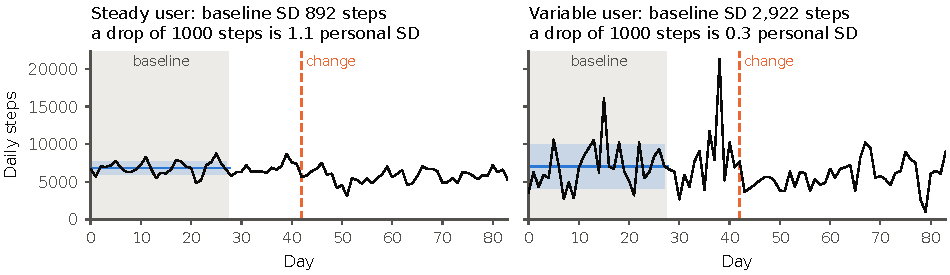
\includegraphics[width=\linewidth]{figures/fig_example.pdf}
  \caption{Two simulated users with the same average level (7\,000 steps) and the same 1000-step drop on day 42. Shading marks the 28-day baseline, the blue band is the baseline mean $\pm$ one personal standard deviation (the SD of the 28 baseline days in steps; the groups in \cref{sec:method} are defined on the log scale). For the steady user the drop exceeds one personal SD; for the variable user it is a third of one.}
  \label{fig:example}
\end{figure}

\section{Related work}
\paragraph{Change detection.}
The fixed-threshold, EWMA and CUSUM detectors we audit are classical tools of sequential monitoring \citep{page1954,roberts1959}. Self-starting variants estimate the baseline from the data themselves \citep{hawkins1987}. Surveys of online change-point detection and of concept drift are given by \citet{aminikhanghahi2017} and \citet{gama2014}. We fix the baseline after 28 days, so slow drift is not adapted to; we return to this in \cref{sec:discussion}.

\paragraph{Personal baselines in wearables.}
Work on pre-symptomatic infection detection from smartwatch data uses each person's own history as the reference \citep{mishra2020,alavi2022}, and \citet{cacheda2026} model deviations from personalised baselines for the early detection of infectious diseases.
The preprint version of \citet{alavi2022} reports an alert rule with a fixed offset above each person's own baseline, and notes that some individuals have a very unstable baseline.\footnote{medRxiv preprint, doi:10.1101/2021.06.13.21258795.}
\citet{morenomunoz2018} detect changes in smartphone data with a hierarchical circadian model, motivated by relapse detection in psychiatric patients.
\citet{tolosa2026} mark a day as a drift day when a composite of per-user rolling z-scores of Fitbit and phone data from university students exceeds a participant-specific quantile threshold; they judge their detectors against proxy labels derived from the same rolling baselines, with precision, recall and AUC.
We did not find in our searches an evaluation of how the alarm rate and detection delay of such detectors depend on a person's own variability; the studies above ask other questions. This was not a systematic review, and not finding a study does not show that none exists.

\paragraph{Equal treatment, shrinkage and evaluation methods.}
\citet{dwork2011} formalise the idea that similar individuals should be treated similarly. Our audit is group-based and descriptive and does not use their framework.
The scale we use in \cref{sec:lambda}, a weighted mixture of an individual and a pooled scale, is in the spirit of the variance shrinkage used in empirical-Bayes analysis of microarray data \citep{smyth2004}, but it is not that method: it mixes standard deviations rather than variances, with a fixed weight rather than one estimated from the data. Its use here is algebraically simple, and what we add is the measured size and shape of its effect on the two definitions of equal treatment.
For the study design we follow the ADEMP structure for simulation studies \citep{morris2019} and the idea of planning and time-stamping a simulation study in advance \citep{siepe2024}, we use an equivalence-style margin to call a gap negligible \citep{lakens2017}, and we use a restricted mean of the delay in the manner of the restricted mean survival time \citep{royston2013}.

\section{Method}\label{sec:method}
\subsection{Setting and groups}
A system observes one value per person per day, here the daily step count $x_t$. Days 0--27 are the baseline; the system may raise alarms from day 28.
A person's variability is the standard deviation of $\log x_t$ over the baseline days. People are split into three equal groups (terciles) by this value; we compare the highest (``high'') with the lowest (``low'') tercile.
The grouping is computed from the same 28 baseline days a deployed system would have, so it is noisy by design.

\subsection{Detectors}
On day $t$ every detector sees only data up to day $t$.
Let $\Delta_t$ be the mean of the last 7 days minus the mean of the 21 days before them (days $t-27$ to $t-7$), and $S_t$ the standard deviation of those 21 days.
Let $u_t=(x_t-m_0)/s_0$ be the day's value standardised by the mean $m_0$ and standard deviation $s_0$ of days 0--27.
\begin{itemize}
  \item \textbf{Fixed threshold:} alarm if $\Delta_t\le -T$, with one $T$ in steps for everyone.
  \item \textbf{Personal z-score:} alarm if $\Delta_t/S_t\le -c$.
  \item \textbf{EWMA:} $z_t=\omega u_t+(1-\omega)z_{t-1}$ with $\omega=0.2$; alarm if $z_t\le -L\sqrt{\omega/(2-\omega)}$.
  \item \textbf{CUSUM (one-sided, downward):} $C_t=\max(0,\,C_{t-1}-u_t-k)$ with $k=0.5$; alarm if $C_t\ge h$.
\end{itemize}
EWMA and CUSUM reset their state to zero after an alarm.
When days are missing, the window detectors abstain unless at least 3 of the last 7 days and at least half of the prior window are observed, EWMA and CUSUM skip the update, and no detector alarms on an unobserved day.
In \cref{sec:lambda} we also use a window detector with a mixed scale: alarm if $\Delta_t/\bigl(\lambda S_t+(1-\lambda)S_{\mathrm{pop}}\bigr)\le -c$, where $S_{\mathrm{pop}}$ is the median of $S_t$ over the windows of the calibration set. With $\lambda=0$ this is a fixed threshold in steps (up to rescaling), with $\lambda=1$ the personal z-score. A robust version replaces $S_t$ by $1.4826$ times the median absolute deviation.
\paragraph{Which spread is used where.}
Three different spreads appear, for three different jobs. The \emph{groups} use the SD of $\log x_t$ over days 0--27, because step counts are skewed and, in our simulator, their spread grows with their level. The \emph{size of a standardised change}, and the scale of EWMA and CUSUM, use the SD in steps of days 0--27, $s_0$: this is what ``one personal standard deviation'' means for a system that fixes its baseline after four weeks. The \emph{z-score} uses the moving SD $S_t$ of the 21 days before the last week, the usual form of ``recent against prior''. These are design choices, not findings. \Cref{sec:fixedscale} checks one of them, a z-score that uses $s_0$ instead of $S_t$.

\subsection{Matched operating point}
Each detector has one tuning constant ($T$, $c$, $L$ or $h$). It is set by bisection on a separate calibration set (different random seed; 101 versus 202 for evaluation) so that the pooled alarm rate over all users and days without a change equals 3.33 alarm episodes per 100 user-days, about one per 30 days. Alarms within 7 days of an earlier alarm form one episode. The constant is the same for all users; the groups are never used for tuning.

\subsection{Injected change and measures}
Each series receives one downward level shift from an onset day drawn uniformly from days 35--49 to the end of the series, floored at zero steps. The un-shifted and shifted versions share the same noise, for every detector. We use two definitions of equal treatment, and report both:
\begin{itemize}
  \item \emph{standardised}: the shift is $k$ times the person's own baseline standard deviation, with $k\in\{0.5,1,1.5,2\}$ and $k=1$ primary;
  \item \emph{absolute}: the shift is the same number of steps for everyone (500 to 2000; 1000 is primary).
\end{itemize}
We measure (i) the \emph{alarm rate}: alarm episodes per 100 user-days on series without a change; (ii) the \emph{delay}: days from onset to the first alarm on or after onset, censored at 14 days, summarised by its mean (restricted mean delay); (iii) \emph{detection within 14 days}: the share of series with an alarm in the first 14 days. Values are averaged over a user's replicates first, so the user is the unit of analysis.

\subsection{Gaps, margins and verdicts}
The gap is the group mean in the high tercile minus that in the low tercile. Intervals are 95\% percentile bootstrap intervals (1000 resamples of users within terciles; the plan said 2000, see \cref{app:timeline}).
A gap is called \emph{meaningful} if its interval excludes zero and the gap exceeds the margin; \emph{negligible} if the whole interval lies inside the margin; \emph{inconclusive} otherwise. These labels describe the interval; they are not tests. ``Meaningful'' does not show that the true gap exceeds the margin, only that the interval excludes zero and the estimate lies beyond the margin. Verdicts use unrounded values. The margins are 1.0 alarm per 100 user-days (30\% of the pooled target), 1.5 days of delay, and 0.10 in the share detected within 14 days. They are judgement calls, not derived from any user or clinical need; they were proposed in the analysis plan before the first run and confirmed unchanged after it.

\subsection{Analysis plan}\label{sec:plan}
The analysis plan was written before the runs and kept, with dated amendments, in the project's git repository; the plan for the real-data check was written before the data were opened. Later experiments were described with their decision rules in amendments before they were run. This is a plan kept by the author in a version-controlled repository, not a registration with an independent registry, and commit times are not an external time stamp. Some analyses were added after earlier results were known; these are labelled as post hoc where they occur, and \cref{app:timeline} lists every deviation from the plan.

\section{Simulation study}\label{sec:sim}
Following ADEMP \citep{morris2019}:
\textbf{Aims}: to compare groups of different day-to-day variability on alarm rate, delay and detection, for four detectors, and to see how the gaps depend on the definition of equal treatment.
\textbf{Data-generating process}: 300 users $\times$ 20 replicates $\times$ 84 days of daily steps. Each user has a level (log-normal, median 7\,000), a log-scale variability $\sigma$ (log-normal across users, median 0.30, clipped to 0.10--0.90), an autocorrelation (uniform 0 to 0.5), and a weekly cycle (amplitude uniform 0 to 0.2). Noise is Student-$t$ with 4 degrees of freedom on the log scale. Full details are in \cref{app:sim}. In the base case (``realistic'') nothing is missing; other scenarios add missing days (more for variable users), shorter windows, symmetric noise, or run the detectors on log steps.
\textbf{Estimands}: the high-minus-low gaps in alarm rate, restricted mean delay and detection within 14 days.
\textbf{Methods}: the four detectors and the mixed-scale family.
\textbf{Performance measures}: the gaps with bootstrap intervals and the verdicts above.
All of this is an assumption set chosen for the audit, not an estimate from real people.

\section{Results in simulation}
\subsection{Audit of the four detectors}\label{sec:audit}
\Cref{tab:audit} and \cref{fig:audit} show the base case.
\paragraph{Fixed threshold.}
High-variability users receive \GrpFixedHighAlarm{} alarm episodes per 100 user-days against \GrpFixedLowAlarm{} for low-variability users (gap \RealFixedAlarmCI). For a change of one personal standard deviation the delay gap is \RealFixedRmdStdCI{} days (the high group is detected sooner) and the gap in the share detected within 14 days is \RealFixedDetStd. These are meaningful gaps; they are expected, because a one-SD change is a larger step for variable users.
\paragraph{Personal-baseline detectors.}
For a change of one personal standard deviation, no delay or detection gap reaches the margin. The delay gaps are \RealZscoreRmdStd{} (z-score), \RealEwmaRmdStd{} (EWMA) and \RealCusumRmdStd{} days (CUSUM), the detection gaps \RealZscoreDetStd, \RealEwmaDetStd{} and \RealCusumDetStd, and all intervals lie inside the margins.
Alarm-rate gaps are \RealZscoreAlarm{} (z-score) and \RealEwmaAlarm{} (EWMA), both negligible, and \RealCusumAlarmCI{} for CUSUM, where the high group gets fewer alarms (\GrpCusumHighAlarm{} against \GrpCusumLowAlarm) and the interval reaches the margin; we call it inconclusive.
\paragraph{The other definition of equal treatment.}
If every user loses the same 1000 steps, the picture changes. The personal detectors are now slower for high-variability users by \RealZscoreRmdAbsCI{} days (z-score), \RealEwmaRmdAbsCI{} (EWMA) and \RealCusumRmdAbsCI{} (CUSUM), and the gaps in the share detected within 14 days are \RealZscoreDetAbs, \RealEwmaDetAbs{} and \RealCusumDetAbs, all meaningful. The fixed threshold has the opposite sign (\RealFixedRmdAbs{} days).
Of the \AuditMeaningful{} meaningful cells in this subsection (the 20 cells of \cref{tab:audit} and of the 1000-step results), \AuditClear{} have an interval that lies entirely beyond its margin.
No detector in this set treats both definitions alike. That is not a defect of a detector: the two definitions disagree because a fixed number of steps is a different multiple of different users' standard deviations.

\begin{table}[t]
\centering
\small
\caption{Audit in the base simulation (``realistic'', 300 users $\times$ 20 replicates). Group means by variability tercile, and the gap (high $-$ low) with its 95\% bootstrap interval. Verdicts follow the margins fixed in advance: 1.0 alarm per 100 user-days, 1.5 days, 0.10 in proportion detected. ``Negligible'' means the whole interval lies inside the margin; ``meaningful'' means the interval excludes zero and the gap exceeds the margin.}
\label{tab:audit}
\begin{tabular}{@{}lrrrlc@{}}
\toprule
Detector & Low & Mid & High & Gap [95\% CI] & Verdict \\
\midrule
\multicolumn{6}{@{}l}{\emph{A. Alarm episodes per 100 user-days, series without a change}} \\
Fixed threshold & 1.87 & 3.32 & 5.20 & +3.33 [+2.81, +3.91] & meaningful \\
Personal z-score & 3.42 & 3.35 & 3.22 & $-$0.21 [$-$0.41, 0.00] & negligible \\
EWMA & 3.45 & 3.35 & 2.98 & $-$0.47 [$-$0.65, $-$0.29] & negligible \\
CUSUM & 3.68 & 3.33 & 2.68 & $-$0.99 [$-$1.22, $-$0.79] & inconclusive \\
\midrule
\multicolumn{6}{@{}l}{\emph{B. Restricted mean delay in days (censored at 14), change of 1 personal SD}} \\
Fixed threshold & 6.69 & 4.54 & 3.31 & $-$3.37 [$-$3.96, $-$2.70] & meaningful \\
Personal z-score & 3.60 & 3.65 & 3.94 & +0.34 [+0.12, +0.55] & negligible \\
EWMA & 2.98 & 3.03 & 3.29 & +0.31 [+0.06, +0.53] & negligible \\
CUSUM & 2.40 & 2.44 & 2.71 & +0.31 [+0.12, +0.51] & negligible \\
\midrule
\multicolumn{6}{@{}l}{\emph{C. Proportion detected within 14 days, change of 1 personal SD}} \\
Fixed threshold & 0.74 & 0.89 & 0.95 & +0.22 [+0.16, +0.27] & meaningful \\
Personal z-score & 0.96 & 0.96 & 0.94 & $-$0.02 [$-$0.04, $-$0.01] & negligible \\
EWMA & 0.97 & 0.97 & 0.95 & $-$0.02 [$-$0.03, $-$0.01] & negligible \\
CUSUM & 0.99 & 0.99 & 0.97 & $-$0.02 [$-$0.03, $-$0.01] & negligible \\
\bottomrule
\end{tabular}
\end{table}


\begin{figure}[t]
  \centering
  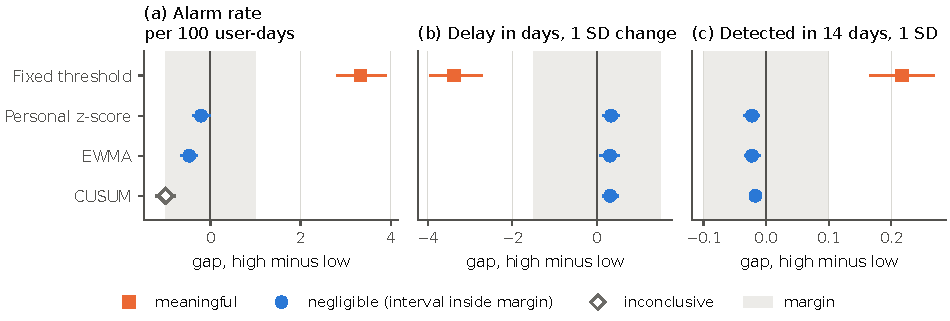
\includegraphics[width=\linewidth]{figures/fig_audit.pdf}
  \caption{Gaps (high minus low variability tercile) with 95\% intervals in the base simulation; same data as \cref{tab:audit}. Shading is the margin. Squares: meaningful; circles: negligible (interval inside the margin); open diamond: inconclusive.}
  \label{fig:audit}
\end{figure}

\subsection{Other simulated scenarios}
\Cref{tab:scenarios} repeats the audit in eight scenarios. In none of them does a personal detector show a meaningful delay or detection gap at any of the four sizes of change (\ScenMeaningfulTotal{} meaningful cells out of 192); the largest delay gap at one personal SD, in absolute value, is \ScenMaxPersonalRmd{} days (\ScenMaxPersonalWhich). The fixed threshold always shows a meaningful alarm-rate gap.
The CUSUM alarm-rate gap is the one personal-detector cell that varies: \ScIdealCusumAlarm{} in the ideal scenario and \ScMissingCusumAlarm{} with missing days (both just beyond the margin), \RealCusumAlarm{} in the base case, and \ScRealLogCusumAlarm{} when the detectors run on log steps or \ScSymmetricCusumAlarm{} with symmetric noise.
In this simulator the gap disappears when skewness is removed. That fits the idea, which we proposed after the first run (a post hoc diagnostic), that it is a side effect of the log-normal model, where variability and skewness grow together. We did not establish the mechanism, and the diagnostic holds only within this simulator.

\begin{table}[t]
\centering
\small
\caption{Alarm-rate gap (high $-$ low tercile, per 100 user-days) in eight simulated scenarios. Bold: the interval excludes zero and the gap exceeds 1.0. Cells: for the three personal-baseline detectors, the number of cells with a meaningful delay or detection gap among 24 (3 detectors $\times$ delay and detection $\times$ four change sizes of 0.5 to 2 personal SD). Max delay gap: the largest delay gap (days) at 1 personal SD.}
\label{tab:scenarios}
\begin{tabular}{@{}p{5.2cm}rrrrrr@{}}
\toprule
 & \multicolumn{4}{c}{Alarm-rate gap} & \multicolumn{2}{c}{Personal detectors} \\
\cmidrule(lr){2-5}\cmidrule(l){6-7}
Scenario & Fixed & z-score & EWMA & CUSUM & Cells & Max delay gap \\
\midrule
Ideal (Gaussian, no autocorrelation, no weekly cycle) & \textbf{+3.64} & $-$0.23 & $-$0.40 & \textbf{$-$1.16} & 0 & $-$0.08 \\
Realistic (base case) & \textbf{+3.33} & $-$0.21 & $-$0.47 & $-$0.99 & 0 & +0.34 \\
Realistic, detectors on log steps & \textbf{+2.96} & +0.13 & $-$0.10 & $-$0.11 & 0 & $-$0.80 \\
Symmetric noise on the raw scale & \textbf{+2.06} & +0.27 & 0.00 & $-$0.03 & 0 & +0.15 \\
Missing days (more for variable users) & \textbf{+3.13} & $-$0.18 & $-$0.63 & \textbf{$-$1.02} & 0 & +0.64 \\
14-day windows & \textbf{+3.20} & $-$0.20 & $-$0.39 & $-$0.68 & 0 & +0.28 \\
7-day windows & \textbf{+3.02} & $-$0.23 & $-$0.26 & $-$0.38 & 0 & +0.23 \\
Missing days and 14-day windows & \textbf{+3.03} & $-$0.16 & $-$0.53 & $-$0.75 & 0 & +0.43 \\
\bottomrule
\end{tabular}
\end{table}


\subsection{Mixing own and population scale}\label{sec:lambda}
\Cref{fig:lambda} shows the mixed-scale detector for $\lambda$ from 0 to 1, each re-tuned to the same alarm rate (\cref{tab:lambda} gives the numbers).
As $\lambda$ rises, the alarm-rate gap falls from \LamSdZeroAlarm{} to \LamSdOneAlarm{}, the delay gap for a change of one personal SD rises from \LamSdZeroRmdStd{} to \LamSdOneRmdStd{} days, and the delay gap for a change of 1000 steps rises from \LamSdZeroRmdAbs{} to \LamSdOneRmdAbs{} days, passing zero near $\lambda=0.5$.
At $\lambda=0.75$ the three gaps are all inside their margins as point estimates: alarm \LamSdThreeQuartersAlarmCI, delay at one SD \LamSdThreeQuartersRmdStdCI{} and at 1000 steps \LamSdThreeQuartersRmdAbsCI{} days; the intervals of the alarm and absolute-delay gaps extend past their margins, so none of the three is called negligible.
The robust scale narrows the delay gaps but leaves a larger alarm-rate gap at the same $\lambda$ (at $\lambda=0.75$: \LamMadThreeQuartersAlarm{} against \LamSdThreeQuartersAlarm).

\paragraph{The trade-off criterion set in the plan was not met.}
Our plan asked whether the gap under the absolute definition grows in size from $\lambda=0$ to $\lambda=1$ by more than 1.5 days while the gap under the standardised definition shrinks by more than 1.5 days. The second holds (the standardised gap goes from \LamSdZeroRmdStd{} to \LamSdOneRmdStd{} days); the first does not: the absolute gap goes from \LamSdZeroRmdAbs{} to \LamSdOneRmdAbs{} days, so it changes sign and its size shrinks instead of growing by more than 1.5. What the data show is a \emph{crossing}, not the trade-off we anticipated. We describe it after the fact and test its robustness in the next section with criteria written before that run.

\begin{figure}[t]
  \centering
  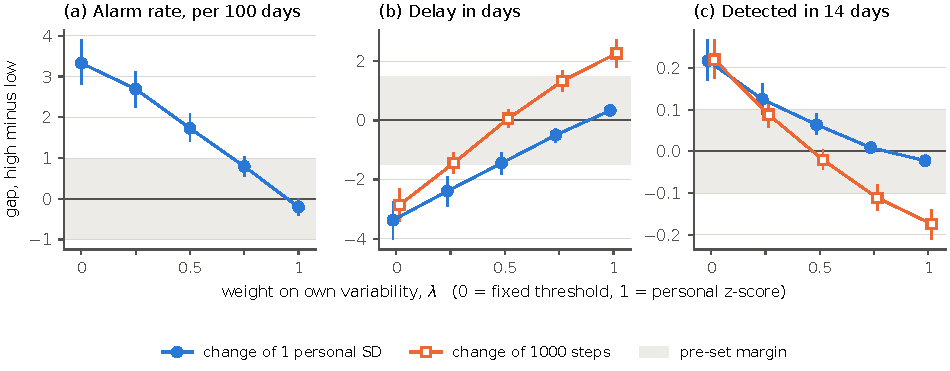
\includegraphics[width=\linewidth]{figures/fig_lambda.pdf}
  \caption{Mixing own and population scale (base simulation, standard-deviation scale). Gaps (high minus low tercile) with 95\% intervals as the weight $\lambda$ on the user's own variability rises from 0 (fixed threshold) to 1 (personal z-score). Shading is the margin. Blue circles: a change of one personal SD; orange squares: a change of 1000 steps (alarm rate: no change).}
  \label{fig:lambda}
\end{figure}

\subsection{Robustness}\label{sec:robust}
Before running them, we fixed three claims and the criteria for each: \textbf{R1}, personal detectors show no meaningful delay or detection gap at one personal SD; \textbf{R2}, the crossing (alarm gap above $+1.0$ at $\lambda=0$ and below $+1.0$ at $\lambda=1$; absolute-change delay gap at most $-1.5$ days at $\lambda=0$ and at least $+1.5$ at $\lambda=1$); \textbf{R3}, some $\lambda$ on the grid has the alarm gap within $\pm1.0$ and both delay gaps within $\pm1.5$ days. We ran them in the base case, in 16 settings that change one assumption at a time (alarm-rate target, seeds, number of users, autocorrelation, spread of variability, tails, correlation of level and variability, shape of the change), and in three settings that change several together (\cref{fig:sens}, \cref{tab:sens}).
\begin{itemize}
  \item \textbf{R1 holds} in \SensRoneOk{} of \SensN{} one-at-a-time settings (\SensRoneLabel) and in \CombRoneOk{} of \CombN{} combined settings, so in all \AllSettings{} settings including the base case. The largest personal-detector delay gap at one personal SD in these \AllSettings{} settings is \SensMaxPersonal{} days in absolute value (CUSUM, widest spread of variability); the eight scenarios of \cref{tab:scenarios} reach \ScenMaxPersonalRmd{} days (\ScenMaxPersonalWhich).
  \item \textbf{R2 holds} in \SensRtwoOk{} of \SensN{} (\SensRtwoLabel) and in \CombRtwoOk{} of \CombN{} combined settings. It fails when the alarm-rate target is raised to 6.0, when the spread of variability is narrow, and when the change is a 14-day ramp. The signs are the same everywhere; only the size falls under the criterion. The size grows with the spread of variability: the alarm gap at $\lambda=0$ is \SSpreadNarrowAlarmZero{} (narrow), \SBaseAlarmZero{} (base) and \SSpreadWideAlarmZero{} (wide).
  \item \textbf{R3 holds} in \SensRthreeOk{} of \SensN{} (\SensRthreeLabel) and in \CombRthreeOk{} of \CombN{} combined settings; the balanced value is $\lambda=\BaseBalanced$ in the base case, and it only just holds. It fails with positive correlation between level and variability, with the widest spread, in the most heterogeneous combination (at $\lambda=0.75$: alarm \CombStressThreeQuartersAlarm, delay \CombStressThreeQuartersRmdStd{} and \CombStressThreeQuartersRmdAbs{} days, all meaningful), and in one evaluation seed by 0.005 days.
\end{itemize}
One of the predictions we wrote before the combined runs was wrong: we expected R2 to hold under the ``real-data-like'' combination and it did not.
Seed-to-seed variation of the delay gap at $\lambda=1$ is about 0.4 days (\SBaseDelayOne, \SEvalSeedADelayOne{} and \SEvalSeedBDelayOne{} for three evaluation seeds).
No setting produces a CUSUM alarm-rate gap as large as the one seen in real data (\cref{sec:ls}): the most negative is \SensMostNegCusum{} per 100 user-days, against \LsCusumAlarmCI{} in the real data.
The reading is: the audit finding R1 is robust in this simulator; the crossing has the same direction everywhere but its size depends on how spread out users' variability is; and a single balanced $\lambda$ is not a stable result.

\begin{figure}[t]
  \centering
  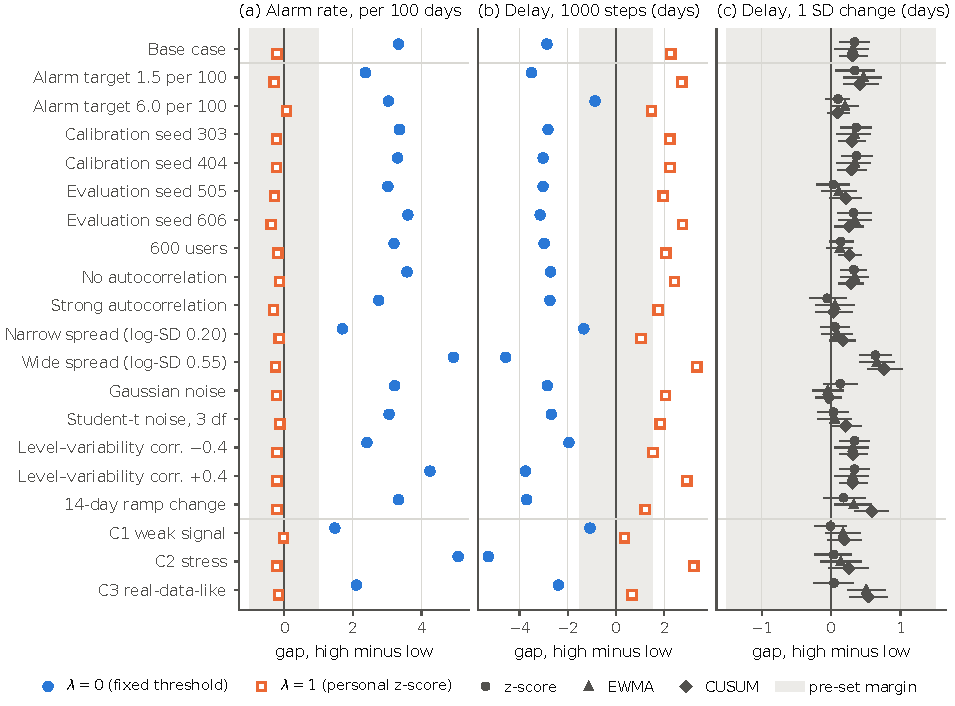
\includegraphics[width=\linewidth]{figures/fig_sensitivity.pdf}
  \caption{Robustness across 20 settings: the base case, 16 settings that change one assumption, and 3 combinations (C1 weak signal, C2 stress, C3 real-data-like; definitions in \cref{app:sim}). (a, b) Gaps at $\lambda=0$ (fixed threshold, blue circles) and $\lambda=1$ (personal z-score, orange squares). (c) Delay gap for a change of one personal SD for the three personal detectors, with 95\% intervals. Shading is the margin. Same data as \cref{tab:sens}.}
  \label{fig:sens}
\end{figure}

\subsection{Does the scale of the z-score matter?}\label{sec:fixedscale}
The z-score divides by the moving SD of the 21 days before the last week, whereas EWMA and CUSUM use the SD of the baseline. To see whether the z-score's pattern depends on that choice, we ran a version, $\mathrm{z}_0$, that divides the same window difference by the baseline SD $s_0$. This check was added after all other results were known, in response to a reader's question; its plan, with three predictions, was written down before it was run (\cref{app:timeline}). It was run in the base simulation and in the simulation with missing days.
All three predictions held in both scenarios. $\mathrm{z}_0$ shows no meaningful delay or detection gap at one personal SD (delay gap \FsRealRmdStdCI{} days in the base case and \FsMissRmdStdCI{} with missing days); its alarm-rate gap is \FsRealAlarmVerdict{} in both (\FsRealAlarmCI{} and \FsMissAlarmCI{}); and it is slower for variable users when every user loses 1000 steps (\FsRealRmdAbsCI{} and \FsMissRmdAbsCI{} days), as the moving-scale z-score is (\cref{tab:fixedscale}). In these two scenarios the z-score's pattern therefore does not depend on which of the two scales it uses. The CUSUM alarm-rate gap (\RealCusumAlarmCI{} in the base case) is not reproduced by $\mathrm{z}_0$, so the use of a baseline scale is not what produces it.

\begin{table}[H]
\centering
\footnotesize
\setlength{\tabcolsep}{3.0pt}
\caption{Personal z-score with the moving scale (SD of the 21 days before the last week) and with the baseline scale (SD of days 0--27, $\mathrm{z}_0$): gap (high $-$ low tercile) with 95\% interval and verdict, for the base simulation and the simulation with missing days. Alarm rate per 100 user-days; delay in days; detection as a proportion within 14 days.}
\label{tab:fixedscale}
\begin{tabular}{@{}lrrl@{}}
\toprule
Measure & z-score (moving scale) & $\mathrm{z}_0$ (baseline scale) & $\mathrm{z}_0$ verdict \\
\midrule
\multicolumn{4}{@{}l}{\emph{Base simulation}} \\
Alarm rate & $-$0.21 [$-$0.41, 0.00] & +0.13 [$-$0.04, +0.34] & negligible \\
Delay, 1 personal SD & +0.34 [+0.12, +0.55] & +0.30 [+0.08, +0.53] & negligible \\
Detected, 1 personal SD & $-$0.02 [$-$0.04, $-$0.01] & $-$0.01 [$-$0.03, 0.00] & negligible \\
Delay, 1000 steps & \textbf{+2.27 [+1.83, +2.73]} & \textbf{+2.06 [+1.63, +2.53]} & meaningful \\
Detected, 1000 steps & \textbf{$-$0.17 [$-$0.21, $-$0.14]} & \textbf{$-$0.17 [$-$0.21, $-$0.13]} & meaningful \\
\midrule
\multicolumn{4}{@{}l}{\emph{Missing days}} \\
Alarm rate & $-$0.18 [$-$0.34, +0.02] & +0.15 [$-$0.03, +0.31] & negligible \\
Delay, 1 personal SD & +0.35 [+0.15, +0.56] & +0.44 [+0.23, +0.66] & negligible \\
Detected, 1 personal SD & $-$0.02 [$-$0.03, $-$0.01] & $-$0.03 [$-$0.04, $-$0.01] & negligible \\
Delay, 1000 steps & \textbf{+2.18 [+1.74, +2.62]} & \textbf{+2.00 [+1.55, +2.45]} & meaningful \\
Detected, 1000 steps & \textbf{$-$0.16 [$-$0.20, $-$0.12]} & \textbf{$-$0.17 [$-$0.21, $-$0.13]} & meaningful \\
\bottomrule
\end{tabular}
\end{table}


\FloatBarrier
\section{Consistency check on real data (LifeSnaps)}\label{sec:ls}
\subsection{Data and procedure}
LifeSnaps \citep{yfantidou2022} is an open dataset of Fitbit and survey data from 71 participants. We used version 4 of the Zenodo record (CC BY 4.0; \citealp{lifesnaps_zenodo}) and only its daily step counts.
A user's day 0 is the first day with a step count above zero. A day with zero steps or no record is treated as not observed (a run that keeps zero-step days is reported below). Days 0--27 are the baseline and days 28 to the last day, at most 56 days, the evaluation segment. A user is eligible with at least 14 observed baseline days, at least 35 evaluation days and at least half of them observed. \LsEligible{} of \LsTotal{} users were eligible, 17 per variability tercile.
The detectors are the same, with the missing-day rules of the simulation. Their constants are set so that the pooled alarm rate on the users' own series equals 3.33 per 100 user-days; there is no separate calibration set and no group information is used in tuning. Each detector has a single constant, fitted on the same users whose group gaps are then measured: the pooled alarm rate is matched in sample by construction and is not a result, while the group gaps are not fitted. This is a descriptive consistency check, not an out-of-sample validation; \cref{sec:crossfit} repeats it with cross-fitted constants. For each user we inject 20 downward level shifts at random onsets and apply the same measures and margins as in simulation. The plan for this check was committed before any data were opened.
Because real series contain real changes, we call the alarm rate here an alarm rate, not a false-alarm rate.

\subsection{Results}
The high-variability tercile has lower median daily steps, a larger share of days without a step count, and a Spearman correlation between log-SD and median steps of \LsSpearman{} (\cref{tab:lsterc}); these are differences between the groups that we report and do not explain.
\Cref{tab:ls} and \cref{fig:ls} compare real-data gaps with the simulated gaps from the matching scenario. The simulated gap lies inside the real-data interval in \LsConsistent{} of \LsCells{} cells, but only \LsInformative{} cells are informative (interval not containing both the simulated gap and zero). The real gap has the same sign as the simulated one in \LsSameSign{} of \LsCells. Intervals are wide: with 17 users per group, an alarm-rate gap is known only to within about $\pm1.5$ to $\pm1.8$ per 100 user-days.
\begin{itemize}
  \item \textbf{Fixed threshold.} The real alarm-rate gap is \LsFixedAlarmCI{} against \LsFixedAlarmSim{} simulated, so the simulated gap is outside the interval. The direction agrees.
  \item \textbf{Personal z-score and EWMA.} Every interval contains zero and the simulated gap, with one exception: the EWMA detection gap for a 1000-step change (\LsEwmaDetAbsCI) is meaningful, as it is in simulation (\LsEwmaDetAbsSim).
  \item \textbf{CUSUM stands out.} The real alarm-rate gap is \LsCusumAlarmCI{} against \LsCusumAlarmSim{} simulated, and the delay gap for one personal SD, \LsCusumRmdStdCI{} days, is by the verdict rule just meaningful: the point estimate (\LsCusumRmdStdExact{} before rounding) is barely above the 1.5-day margin and the interval's lower end is close to zero (\LsCusumRmdStdSim{} simulated). The upper end of the alarm-rate interval lies close to the most negative simulated gap in any setting (\cref{sec:robust}), so this is a difference in the point estimate, with a wide interval, and not a firm contradiction of the simulator.
\end{itemize}
In an exploratory run on log steps (post hoc), the simulated CUSUM alarm gap vanishes (\LsLogCusumAlarmSim{}) but the real one does not (\LsLogCusumAlarmCI{}; EWMA \LsLogEwmaAlarmCI{}, simulated \LsLogEwmaAlarmSim), while the CUSUM delay gaps disappear (\LsLogCusumRmdStdCI{} days at one SD). The skewness explanation from the simulator therefore does not explain the real alarm-rate gap. A simulated slow drift away from the baseline, tested with a rule set in advance, did not produce it either (\cref{app:drift}). Keeping zero-step days as observed (\LsZeroEligible{} eligible users) gave \LsZeroConsistent{} of \LsZeroCells{} consistent cells, \LsZeroInformative{} informative, and a CUSUM alarm gap of \LsZeroCusumAlarmCI.
We have not tested the remaining candidates: real changes in the series counted as alarms, wear-time and routine differences tied to variability, and chance with 17 users per group.

\subsection{Tuning on the same users}\label{sec:crossfit}
A reader pointed out that the constants were tuned on the same users whose gaps are evaluated. We therefore added a cross-fitted version after all other results were known; its plan, with two predictions, was written down before it was run (\cref{app:timeline}). Users were split into two folds, at random within each variability tercile (\CfFoldA{} and \CfFoldB{} users). Each detector's constant was tuned to 3.33 per 100 user-days on the users of one fold and applied to the users of the other, and the gaps were computed over all users as before (\cref{tab:crossfit}).
Both predictions held. No cell that was meaningful in sample changed sign (\CfRealKeepSign{} of \CfRealN), and the CUSUM alarm-rate gap stayed large (\CfCusumAlarmCI{} against \LsCusumAlarmCI{} in sample). Verdicts that sit at a margin are not stable, however: \CfVerdictChanges{} of the \CfCells{} verdicts change. The CUSUM delay gap at one personal SD becomes \CfCusumRmdStdCI{} days and is no longer beyond the 1.5-day margin; the EWMA gap in detection within 14 days at 1000 steps (\CfEwmaDetAbsCI) becomes inconclusive; and the z-score gap in the same measure (\CfZscoreDetAbsCI) becomes meaningful. Among the other \CfOtherN{} cells, \CfOtherFlips{} changes sign (a gap near zero). Pooled alarm rates in the held-out folds ranged from \CfPooledMin{} to \CfPooledMax{} per 100 user-days. Constants estimated on about 25 users are noisy, so this check does not turn the LifeSnaps check into an out-of-sample validation; it shows that the sign of the large gaps does not come from tuning on the same users.

\begin{table}[t]
\centering
\small
\caption{LifeSnaps users by variability tercile (log-scale SD of daily steps over the 28 baseline days).}
\label{tab:lsterc}
\begin{tabular}{@{}lrrrrr@{}}
\toprule
Tercile & Users & Median daily steps & Days without a record & Median log-SD & Mean evaluation days \\
\midrule
Low & 17 & 8\,726 & 0.139 & 0.40 & 48.4 \\
Mid & 17 & 6\,878 & 0.144 & 0.61 & 49.9 \\
High & 17 & 6\,292 & 0.175 & 0.93 & 52.2 \\
\bottomrule
\end{tabular}
\end{table}

\begin{table}[t]
\centering
\small
\caption{LifeSnaps consistency check, 51 eligible users, 17 per variability tercile. Real-data gap (high $-$ low) with 95\% interval, next to the gap found in the simulation with missing days. Alarm rate in episodes per 100 user-days (these alarms may include real changes); delay in days for an injected change of 1 personal SD or 1000 steps. Bold: meaningful by the verdict rule. \emph{In}: the simulated gap lies inside the real-data interval.}
\label{tab:ls}
\begin{tabular}{@{}llrlrc@{}}
\toprule
Measure & Detector & Real gap [95\% CI] & & Simulated & In \\
\midrule
Alarm rate & Fixed threshold & +0.84 [$-$0.78, +2.62] & & +3.13 & no \\
 & Personal z-score & $-$0.54 [$-$1.96, +1.01] & & $-$0.18 & yes \\
 & EWMA & $-$0.69 [$-$2.48, +1.13] & & $-$0.63 & yes \\
 & CUSUM & \textbf{$-$3.33 [$-$4.86, $-$1.62]} & & $-$1.02 & no \\
\addlinespace
Delay, 1 personal SD & Fixed threshold & $-$1.01 [$-$2.29, +0.28] & & $-$3.22 & no \\
 & Personal z-score & +0.39 [$-$0.81, +1.64] & & +0.35 & yes \\
 & EWMA & +0.94 [$-$0.68, +2.64] & & +0.58 & yes \\
 & CUSUM & \textbf{+1.50 [+0.21, +3.00]} & & +0.64 & yes \\
\addlinespace
Delay, 1000 steps & Fixed threshold & $-$1.45 [$-$3.61, +0.59] & & $-$2.67 & yes \\
 & Personal z-score & +1.46 [$-$0.63, +3.65] & & +2.18 & yes \\
 & EWMA & +2.29 [$-$0.44, +4.77] & & +2.89 & yes \\
 & CUSUM & \textbf{+3.29 [+0.85, +5.45]} & & +3.27 & yes \\
\bottomrule
\end{tabular}
\end{table}

\begin{table}[!htbp]
\centering
\scriptsize
\setlength{\tabcolsep}{3.0pt}
\caption{LifeSnaps: gaps (high $-$ low tercile) with the tuning constants fitted on all 51 users (in sample, \cref{tab:ls}) and cross-fitted (each user's detectors tuned on the other half of the users). Alarm rate per 100 user-days; delay in days; detection as a proportion within 14 days. Bold: meaningful.}
\label{tab:crossfit}
\begin{tabular}{@{}llrlrl@{}}
\toprule
Detector & Measure & In sample [95\% CI] & Verdict & Cross-fitted [95\% CI] & Verdict \\
\midrule
Fixed threshold & Alarm rate & +0.84 [$-$0.78, +2.62] & inconclusive & +0.70 [$-$0.77, +2.16] & inconclusive \\
 & Delay, 1 personal SD & $-$1.01 [$-$2.29, +0.28] & inconclusive & $-$1.00 [$-$2.29, +0.33] & inconclusive \\
 & Detected, 1 personal SD & +0.05 [$-$0.04, +0.14] & inconclusive & +0.06 [$-$0.04, +0.14] & inconclusive \\
 & Delay, 1000 steps & $-$1.45 [$-$3.61, +0.59] & inconclusive & $-$1.37 [$-$3.52, +0.61] & inconclusive \\
 & Detected, 1000 steps & +0.16 [$-$0.02, +0.34] & inconclusive & +0.14 [$-$0.05, +0.33] & inconclusive \\
\addlinespace
Personal z-score & Alarm rate & $-$0.54 [$-$1.96, +1.01] & inconclusive & +0.14 [$-$1.42, +1.73] & inconclusive \\
 & Delay, 1 personal SD & +0.39 [$-$0.81, +1.64] & inconclusive & +0.56 [$-$0.75, +1.89] & inconclusive \\
 & Detected, 1 personal SD & 0.00 [$-$0.07, +0.06] & negligible & $-$0.01 [$-$0.07, +0.06] & negligible \\
 & Delay, 1000 steps & +1.46 [$-$0.63, +3.65] & inconclusive & +1.60 [$-$0.69, +4.10] & inconclusive \\
 & Detected, 1000 steps & $-$0.17 [$-$0.35, +0.03] & inconclusive & \textbf{$-$0.20 [$-$0.38, 0.00]} & meaningful \\
\addlinespace
EWMA & Alarm rate & $-$0.69 [$-$2.48, +1.13] & inconclusive & $-$0.90 [$-$2.74, +0.97] & inconclusive \\
 & Delay, 1 personal SD & +0.94 [$-$0.68, +2.64] & inconclusive & +1.06 [$-$0.55, +2.76] & inconclusive \\
 & Detected, 1 personal SD & $-$0.05 [$-$0.13, +0.02] & inconclusive & $-$0.06 [$-$0.14, 0.00] & inconclusive \\
 & Delay, 1000 steps & +2.29 [$-$0.44, +4.77] & inconclusive & +2.11 [$-$0.58, +4.71] & inconclusive \\
 & Detected, 1000 steps & \textbf{$-$0.26 [$-$0.45, $-$0.04]} & meaningful & $-$0.24 [$-$0.44, 0.00] & inconclusive \\
\addlinespace
CUSUM & Alarm rate & \textbf{$-$3.33 [$-$4.86, $-$1.62]} & meaningful & \textbf{$-$2.98 [$-$4.50, $-$1.19]} & meaningful \\
 & Delay, 1 personal SD & \textbf{+1.50 [+0.21, +3.00]} & meaningful & +1.41 [+0.16, +2.88] & inconclusive \\
 & Detected, 1 personal SD & $-$0.08 [$-$0.18, 0.00] & inconclusive & $-$0.08 [$-$0.17, 0.00] & inconclusive \\
 & Delay, 1000 steps & \textbf{+3.29 [+0.85, +5.45]} & meaningful & \textbf{+3.74 [+1.46, +5.80]} & meaningful \\
 & Detected, 1000 steps & \textbf{$-$0.30 [$-$0.45, $-$0.14]} & meaningful & \textbf{$-$0.35 [$-$0.51, $-$0.20]} & meaningful \\
\bottomrule
\end{tabular}
\end{table}


\begin{figure}[t]
  \centering
  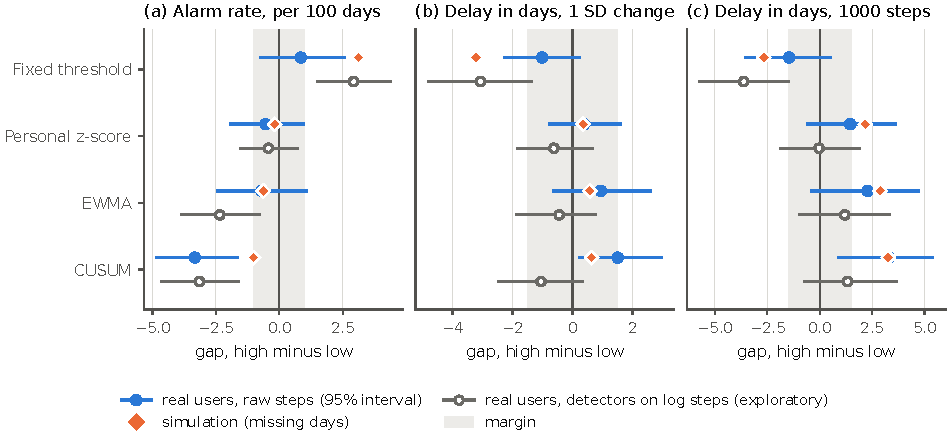
\includegraphics[width=\linewidth]{figures/fig_lifesnaps.pdf}
  \caption{Real-data gaps (high minus low tercile, 17 users each) with 95\% intervals (blue), the matching simulated gap (orange diamonds), and an exploratory run with detectors on log steps (grey, open). Shading is the margin. Same data as \cref{tab:ls}.}
  \label{fig:ls}
\end{figure}

\section{Discussion}\label{sec:discussion}
\paragraph{What the results say.}
In simulation, scaling the alarm by each person's own variability removes the gap in delay and detection when the change is measured in personal standard deviations. It does not remove it when the change is measured in steps: then the people whose days vary most are detected later. This holds whether the z-score divides by a moving or by a baseline scale (\cref{sec:fixedscale}). A fixed threshold does the opposite. The two views cannot both be met by one rule, and a rule that mixes own and population scale can only choose a compromise, which in our simulation exists when users' variability is not too spread out.

\paragraph{For people who build such systems.}
First, report operating characteristics by variability group, not only pooled: pooled alarm rates and mean delays hide the difference. Second, decide and state which promise is being kept: the same sensitivity relative to one's own variability, or the same sensitivity to an absolute change. Third, if a mixed scale is used, treat $\lambda$ as a design choice to be set from what an error costs, not from our simulation: the balanced value we found is specific to our assumptions about users. Fourth, step counts are skewed; the simulation suggests that running CUSUM or EWMA on log steps removes one artefact (the CUSUM alarm gap), though not the one we see in real data.

\paragraph{Limitations.}
\begin{itemize}
  \item The main evidence is a simulator whose assumptions we chose: log-normal users, independent attributes, abrupt level shifts, one signal (daily steps), downward changes only. The sensitivity analysis varies many of these but not all, and 20 settings are not a search of the space.
  \item Only 17 users per tercile are in the real-data check, the changes there are injected, and genuine changes in the series are unlabelled; the check cannot confirm or refute the simulated findings. Its constants were tuned on the same users; a cross-fitted version (\cref{sec:crossfit}) keeps the signs of the large gaps but not every verdict at a margin.
  \item Variability groups are estimated from 28 days and are noisy; the margins are judgement calls. The verdict labels are descriptive, not tests: in the base-simulation audit (\cref{sec:audit}), \AuditClear{} of \AuditMeaningful{} meaningful cells lie entirely beyond their margins, but in the LifeSnaps check only \LsClear{} of \LsMeaningful{} do.
  \item The groups are defined on the log-scale SD, whereas the standardised change and the scale of EWMA and CUSUM use the SD in steps (\cref{sec:method}); we did not vary the grouping variable.
  \item Changes of 1--2 personal SD are floored at zero steps for very variable users (at 2 SD, 40\% of post-onset days in the high tercile against 5\% in the low tercile in the base case), which is why one personal SD is the primary size.
  \item The gap between the two definitions of equal treatment is partly algebraic: a fixed shift is a different multiple of different users' standard deviations. What we add is its size and shape, the matched-alarm-rate protocol, and the check of how far it holds.
  \item We did not study demographic groups; variability may be correlated with age, work or health, and we do not know whether it is. ``Fair'' is used descriptively; we link the gaps to no harm.
  \item The real CUSUM alarm-rate gap is unexplained.
\end{itemize}

\paragraph{Next steps.}
The natural next step is a dataset with labelled events (for example illness onsets) and several signals such as heart rate and sleep, to measure delay on real changes and to test the same audit per person rather than per tercile. Adaptive baselines that follow slow drift \citep{gama2014} should be audited in the same way.

\FloatBarrier
\section{Reproducibility}\label{sec:reproducibility}
\paragraph{Code and results.}
All simulation code, the dated plans, and every result file are in \repo{} (directory \texttt{pilot/}); the results reported here are at commit \commit{}, and the repository is archived on Zenodo as \zenodoDOI. The tables and figures of this paper are generated from the result files by scripts in \texttt{paper/scripts/}, and every number in the text is a macro defined from those files. No special hardware is needed.
\paragraph{Data.}
LifeSnaps is public under CC BY 4.0 \citep{lifesnaps_zenodo}. The data files are not redistributed in the repository; only code and aggregated results are. We did not try to identify any participant.
\paragraph{Deviations from the plan.}
Several analyses were added after earlier results were seen, one of them in response to a real-data result, and the bootstrap used 1000 instead of the planned 2000 resamples (a re-run with 10\,000 changes no point estimate and \McChanges{} of \McWithVerdict{} verdicts). \Cref{app:timeline} lists all deviations, post hoc elements and commit times.

\bibliographystyle{plainnat}
\bibliography{references}

\appendix
\FloatBarrier
\section{Simulator and tuned constants}\label{app:sim}
\paragraph{Users and series.}
For user $i$ and replicate $r$, with $y_t=\log(\mu_i)+w_t+\varepsilon_t$ and $x_t=\exp(y_t)$ steps. Level: $\log\mu_i\sim N(\log 7000,\,0.35^2)$. Variability: $\log\sigma_i\sim N(\log 0.30,\,s^2)$ with $s=0.35$, clipped to $\sigma_i\in[0.10,0.90]$. Noise: AR(1) with coefficient $\phi_i\sim U(0,0.5)$ and stationary standard deviation $\sigma_i$, with innovations Student-$t$ with 4 degrees of freedom scaled to unit variance. Weekly cycle: $w_t=a_i\cos\bigl(2\pi(d_t-\psi_i)/7\bigr)$ with $a_i\sim U(0,0.2)$, $\psi_i\sim U(0,7)$ and a random weekday offset per replicate. The ``ideal'' scenario has Gaussian innovations, $\phi_i=0$ and no weekly cycle. Series have 84 days; evaluation days are 28 to 83; the change starts on a day uniform in 35--49. Variability terciles use the log-scale SD of days 0--27 of the first replicate.
\paragraph{Scenarios.}
\emph{Symmetric}: noise added on the raw scale with relative SD capped at 0.45 and values floored at 5\% of the user's level. \emph{Log steps}: detectors on $\log x_t$. \emph{Missing}: each day is missing with probability $0.05+0.30(\sigma_i-0.10)/0.80$. \emph{Short windows}: prior window and baseline of 14 or 7 days. \emph{Drift}: a linear trend on the log scale reaching $N(0,d^2)$ on day 83, independent of $\sigma_i$.
\paragraph{Sensitivity settings.}
One at a time: alarm target 1.5 or 6.0 (base 3.33); calibration seeds 303 and 404; evaluation seeds 505 and 606; 600 users; $\phi_i$ none or $U(0.3,0.8)$; $s=0.20$ or $0.55$; Student-$t$ with 3 degrees of freedom or Gaussian; correlation of $\log\mu_i$ with $\log\sigma_i$ of $-0.4$ or $+0.4$; a 14-day linear ramp from zero to the full shift. Combined: C1, $s=0.20$, target 6.0 and a 14-day ramp; C2, $s=0.55$, correlation $+0.4$, $t_3$ noise and $\phi_i\sim U(0.3,0.8)$; C3, missing days, 14-day windows, correlation $-0.4$ and a 14-day ramp.
\paragraph{Tuned constants in the base case.}
Fixed $T=1450$ steps, z-score $c=0.584$, EWMA $L=1.29$, CUSUM $h=1.53$; pooled alarm rates on the evaluation set 3.46, 3.33, 3.26 and 3.23 per 100 user-days against a target of 3.33. The population scale for the mixed detector is 2103 steps (standard deviation) or 1711 (robust).

\section{Full tables}
\begin{table}[H]
\centering
\small
\caption{Mixing own and population scale (base simulation). Point estimates of the gap (high $-$ low tercile); bold: meaningful by the pre-set rule. Intervals for every cell are in \cref{tab:lambda_ci}. $\lambda=0$ is a fixed threshold, $\lambda=1$ the personal z-score; each $\lambda$ is re-tuned to the same pooled alarm rate. Delay in days; detection as a proportion.}
\label{tab:lambda}
\begin{tabular}{@{}lrrrrr@{}}
\toprule
 & Alarm rate & \multicolumn{2}{c}{Delay} & \multicolumn{2}{c}{Detected in 14 days} \\
\cmidrule(lr){3-4}\cmidrule(l){5-6}
$\lambda$ & per 100 days & 1 SD & 1000 steps & 1 SD & 1000 steps \\
\midrule
\multicolumn{6}{@{}l}{\emph{Scale: standard deviation}} \\
0 & \textbf{+3.33} & \textbf{$-$3.37} & \textbf{$-$2.86} & \textbf{+0.22} & \textbf{+0.22} \\
0.25 & \textbf{+2.70} & \textbf{$-$2.39} & $-$1.44 & \textbf{+0.12} & +0.09 \\
0.5 & \textbf{+1.73} & $-$1.44 & +0.06 & +0.06 & $-$0.02 \\
0.75 & +0.79 & $-$0.49 & +1.33 & +0.01 & \textbf{$-$0.11} \\
1 & $-$0.21 & +0.34 & \textbf{+2.27} & $-$0.02 & \textbf{$-$0.17} \\
\midrule
\multicolumn{6}{@{}l}{\emph{Scale: robust (1.4826 $\times$ MAD)}} \\
0 & \textbf{+3.33} & \textbf{$-$3.37} & \textbf{$-$2.86} & \textbf{+0.22} & \textbf{+0.22} \\
0.25 & \textbf{+2.89} & \textbf{$-$2.57} & \textbf{$-$1.72} & \textbf{+0.14} & \textbf{+0.11} \\
0.5 & \textbf{+2.28} & \textbf{$-$1.79} & $-$0.69 & +0.09 & +0.02 \\
0.75 & \textbf{+1.55} & $-$1.10 & +0.31 & +0.04 & $-$0.04 \\
1 & +0.72 & $-$0.36 & +1.18 & +0.01 & $-$0.09 \\
\bottomrule
\end{tabular}
\end{table}

\begin{table}[H]
\centering
\scriptsize
\caption{Robustness of the simulation findings across 20 settings: the base case, 16 settings that change one assumption, and 3 that change several together. R1: no meaningful delay or detection gap for the three personal detectors at 1 personal SD. R2: the crossing (alarm gap above $+1.0$ at $\lambda=0$ and below $+1.0$ at $\lambda=1$; absolute-change delay gap at most $-1.5$ days at $\lambda=0$ and at least $+1.5$ at $\lambda=1$). R3: some $\lambda$ on the grid has the alarm gap within $\pm 1.0$ and both delay gaps within $\pm 1.5$ days (the $\lambda$ values are listed). Gaps are high $-$ low tercile; alarm gaps per 100 user-days, delay gaps in days for a 1000-step change. CUSUM: alarm-rate gap of the CUSUM detector.}
\label{tab:sens}
\begin{tabular}{@{}lcccrrrrr@{}}
\toprule
 & & & & \multicolumn{2}{c}{Alarm gap} & \multicolumn{2}{c}{Delay gap, 1000 steps} & \\
\cmidrule(lr){5-6}\cmidrule(lr){7-8}
Setting & R1 & R2 & R3 ($\lambda$) & $\lambda=0$ & $\lambda=1$ & $\lambda=0$ & $\lambda=1$ & CUSUM \\
\midrule
Base case & yes & yes & 0.75 & +3.33 & $-$0.21 & $-$2.86 & +2.27 & $-$0.99 \\
Alarm target 1.5 per 100 & yes & yes & 0.75 & +2.37 & $-$0.29 & $-$3.50 & +2.73 & $-$0.59 \\
Alarm target 6.0 per 100 & yes & \textbf{no} & 0.75, 1 & +3.03 & +0.07 & $-$0.86 & +1.47 & $-$1.07 \\
Calibration seed 303 & yes & yes & 0.75 & +3.36 & $-$0.22 & $-$2.81 & +2.24 & $-$0.96 \\
Calibration seed 404 & yes & yes & 0.75 & +3.30 & $-$0.22 & $-$3.02 & +2.24 & $-$0.95 \\
Evaluation seed 505 & yes & yes & 0.75 & +3.02 & $-$0.28 & $-$3.02 & +1.96 & $-$0.73 \\
Evaluation seed 606 & yes & yes & \textbf{none} & +3.60 & $-$0.38 & $-$3.14 & +2.76 & $-$1.12 \\
600 users & yes & yes & 0.75 & +3.20 & $-$0.19 & $-$2.98 & +2.07 & $-$0.88 \\
No autocorrelation & yes & yes & 0.75 & +3.58 & $-$0.13 & $-$2.71 & +2.43 & $-$1.11 \\
Strong autocorrelation & yes & yes & 0.75 & +2.75 & $-$0.31 & $-$2.74 & +1.75 & $-$0.67 \\
Narrow spread (log-SD 0.20) & yes & \textbf{no} & 0.5, 0.75, 1 & +1.69 & $-$0.14 & $-$1.33 & +1.04 & $-$0.51 \\
Wide spread (log-SD 0.55) & yes & yes & \textbf{none} & +4.93 & $-$0.25 & $-$4.56 & +3.35 & $-$1.52 \\
Gaussian noise & yes & yes & 0.75 & +3.22 & $-$0.23 & $-$2.84 & +2.06 & $-$0.92 \\
Student-t noise, 3 df & yes & yes & 0.75 & +3.05 & $-$0.13 & $-$2.68 & +1.84 & $-$0.79 \\
Level-variability corr. $-0.4$ & yes & yes & 0.75 & +2.41 & $-$0.21 & $-$1.95 & +1.54 & $-$0.99 \\
Level-variability corr. $+0.4$ & yes & yes & \textbf{none} & +4.24 & $-$0.21 & $-$3.75 & +2.94 & $-$0.99 \\
14-day ramp change & yes & \textbf{no} & 0.75, 1 & +3.33 & $-$0.21 & $-$3.70 & +1.21 & $-$0.99 \\
\midrule
C1 weak signal & yes & \textbf{no} & 0.5, 0.75, 1 & +1.48 & $-$0.02 & $-$1.07 & +0.35 & $-$0.52 \\
C2 stress & yes & yes & \textbf{none} & +5.07 & $-$0.21 & $-$5.29 & +3.23 & $-$0.84 \\
C3 real-data-like & yes & \textbf{no} & 0.75, 1 & +2.10 & $-$0.16 & $-$2.39 & +0.66 & $-$0.75 \\
\bottomrule
\end{tabular}
\end{table}

{\footnotesize\setlength{\tabcolsep}{2.4pt}
\begin{longtable}{@{}lllrlrcc@{}}
\caption{All 35 cells of the LifeSnaps check (0-step days treated as not observed). Real-data gap (high $-$ low) with 95\% interval and pre-set verdict; simulated gap in the matching ``missing'' scenario; \emph{Sim.\ in CI}: the simulated gap lies inside the real-data interval; \emph{Informative}: the interval does not contain both the simulated gap and zero.}\label{tab:lsfull}\\
\toprule Detector & Change & Metric & Real gap [95\% CI] & Verdict & Simulated & Sim.\ in CI & Informative \\ \midrule \endfirsthead
\toprule Detector & Change & Metric & Real gap [95\% CI] & Verdict & Simulated & Sim.\ in CI & Informative \\ \midrule \endhead
\bottomrule \endlastfoot
Fixed threshold & none & alarm rate & +0.84 [$-$0.78, +2.62] & inconclusive & +3.13 & no & yes \\
Fixed threshold & 1 SD & delay & $-$1.01 [$-$2.29, +0.28] & inconclusive & $-$3.22 & no & yes \\
Fixed threshold & 1 SD & det. 14 d & +0.05 [$-$0.04, +0.14] & inconclusive & +0.22 & no & yes \\
Fixed threshold & 1000 steps & delay & $-$1.45 [$-$3.61, +0.59] & inconclusive & $-$2.67 & yes & no \\
Fixed threshold & 1000 steps & det. 14 d & +0.16 [$-$0.02, +0.34] & inconclusive & +0.21 & yes & no \\
Personal z-score & none & alarm rate & $-$0.54 [$-$1.96, +1.01] & inconclusive & $-$0.18 & yes & no \\
Personal z-score & 1 SD & delay & +0.39 [$-$0.81, +1.64] & inconclusive & +0.35 & yes & no \\
Personal z-score & 1 SD & det. 14 d & 0.00 [$-$0.07, +0.06] & negligible & $-$0.02 & yes & no \\
Personal z-score & 1000 steps & delay & +1.46 [$-$0.63, +3.65] & inconclusive & +2.18 & yes & no \\
Personal z-score & 1000 steps & det. 14 d & $-$0.17 [$-$0.35, +0.03] & inconclusive & $-$0.16 & yes & no \\
EWMA & none & alarm rate & $-$0.69 [$-$2.48, +1.13] & inconclusive & $-$0.63 & yes & no \\
EWMA & 1 SD & delay & +0.94 [$-$0.68, +2.64] & inconclusive & +0.58 & yes & no \\
EWMA & 1 SD & det. 14 d & $-$0.05 [$-$0.13, +0.02] & inconclusive & $-$0.03 & yes & no \\
EWMA & 1000 steps & delay & +2.29 [$-$0.44, +4.77] & inconclusive & +2.89 & yes & no \\
EWMA & 1000 steps & det. 14 d & $-$0.26 [$-$0.45, $-$0.04] & meaningful & $-$0.20 & yes & yes \\
CUSUM & none & alarm rate & $-$3.33 [$-$4.86, $-$1.62] & meaningful & $-$1.02 & no & yes \\
CUSUM & 1 SD & delay & +1.50 [+0.21, +3.00] & meaningful & +0.64 & yes & yes \\
CUSUM & 1 SD & det. 14 d & $-$0.08 [$-$0.18, 0.00] & inconclusive & $-$0.02 & yes & no \\
CUSUM & 1000 steps & delay & +3.29 [+0.85, +5.45] & meaningful & +3.27 & yes & yes \\
CUSUM & 1000 steps & det. 14 d & $-$0.30 [$-$0.45, $-$0.14] & meaningful & $-$0.23 & yes & yes \\
Mixed scale $\lambda=0$ & none & alarm rate & +0.84 [$-$0.83, +2.62] & inconclusive & +3.13 & no & yes \\
Mixed scale $\lambda=0$ & 1 SD & delay & $-$1.01 [$-$2.22, +0.31] & inconclusive & $-$3.22 & no & yes \\
Mixed scale $\lambda=0$ & 1 SD & det. 14 d & +0.05 [$-$0.04, +0.14] & inconclusive & +0.22 & no & yes \\
Mixed scale $\lambda=0$ & 1000 steps & delay & $-$1.45 [$-$3.47, +0.74] & inconclusive & $-$2.67 & yes & no \\
Mixed scale $\lambda=0$ & 1000 steps & det. 14 d & +0.16 [$-$0.03, +0.35] & inconclusive & +0.21 & yes & no \\
Mixed scale $\lambda=0.5$ & none & alarm rate & +0.50 [$-$0.96, +2.01] & inconclusive & +1.68 & yes & no \\
Mixed scale $\lambda=0.5$ & 1 SD & delay & $-$0.21 [$-$1.57, +1.10] & inconclusive & $-$1.29 & yes & no \\
Mixed scale $\lambda=0.5$ & 1 SD & det. 14 d & +0.01 [$-$0.06, +0.08] & negligible & +0.07 & yes & no \\
Mixed scale $\lambda=0.5$ & 1000 steps & delay & +0.09 [$-$2.01, +2.27] & inconclusive & +0.10 & yes & no \\
Mixed scale $\lambda=0.5$ & 1000 steps & det. 14 d & +0.01 [$-$0.18, +0.20] & inconclusive & $-$0.02 & yes & no \\
Mixed scale $\lambda=1$ & none & alarm rate & $-$0.54 [$-$1.99, +0.89] & inconclusive & $-$0.18 & yes & no \\
Mixed scale $\lambda=1$ & 1 SD & delay & +0.39 [$-$0.91, +1.71] & inconclusive & +0.35 & yes & no \\
Mixed scale $\lambda=1$ & 1 SD & det. 14 d & 0.00 [$-$0.07, +0.06] & negligible & $-$0.02 & yes & no \\
Mixed scale $\lambda=1$ & 1000 steps & delay & +1.46 [$-$0.67, +3.63] & inconclusive & +2.18 & yes & no \\
Mixed scale $\lambda=1$ & 1000 steps & det. 14 d & $-$0.17 [$-$0.34, +0.01] & inconclusive & $-$0.16 & yes & no \\
\end{longtable}
}


\section{Intervals for the tables of the main text}\label{app:intervals}
\begin{table}[!htbp]
\centering
\scriptsize
\setlength{\tabcolsep}{3.0pt}
\caption{Alarm-rate gap (high $-$ low tercile, per 100 user-days) with 95\% interval in the eight simulated scenarios of \cref{tab:scenarios}. Bold: meaningful by the verdict rule.}
\label{tab:scenarios_ci}
\begin{tabular}{@{}p{3.0cm}rrrr@{}}
\toprule
Scenario & Fixed & Personal z-score & EWMA & CUSUM \\
\midrule
Ideal & \textbf{+3.64 [+3.09, +4.14]} & $-$0.23 [$-$0.34, $-$0.13] & $-$0.40 [$-$0.57, $-$0.25] & \textbf{$-$1.16 [$-$1.35, $-$1.00]} \\
Base case & \textbf{+3.33 [+2.81, +3.91]} & $-$0.21 [$-$0.41, 0.00] & $-$0.47 [$-$0.65, $-$0.29] & $-$0.99 [$-$1.22, $-$0.79] \\
Detectors on log steps & \textbf{+2.96 [+2.67, +3.24]} & +0.13 [$-$0.05, +0.32] & $-$0.10 [$-$0.27, +0.07] & $-$0.11 [$-$0.30, +0.08] \\
Symmetric noise & \textbf{+2.06 [+1.57, +2.52]} & +0.27 [+0.08, +0.46] & 0.00 [$-$0.19, +0.18] & $-$0.03 [$-$0.21, +0.16] \\
Missing days & \textbf{+3.13 [+2.63, +3.66]} & $-$0.18 [$-$0.34, +0.02] & $-$0.63 [$-$0.80, $-$0.47] & \textbf{$-$1.02 [$-$1.21, $-$0.82]} \\
14-day windows & \textbf{+3.20 [+2.69, +3.74]} & $-$0.20 [$-$0.40, +0.02] & $-$0.39 [$-$0.58, $-$0.20] & $-$0.68 [$-$0.89, $-$0.47] \\
7-day windows & \textbf{+3.02 [+2.52, +3.51]} & $-$0.23 [$-$0.44, $-$0.01] & $-$0.26 [$-$0.47, $-$0.04] & $-$0.38 [$-$0.61, $-$0.14] \\
Missing days, 14-day windows & \textbf{+3.03 [+2.54, +3.54]} & $-$0.16 [$-$0.34, +0.05] & $-$0.53 [$-$0.71, $-$0.33] & $-$0.75 [$-$0.97, $-$0.55] \\
\bottomrule
\end{tabular}
\end{table}
\begin{table}[!htbp]
\centering
\footnotesize
\setlength{\tabcolsep}{3.0pt}
\caption{Delay gap (days, high $-$ low tercile) for a change of one personal SD, with 95\% interval, in the eight simulated scenarios; the three personal-baseline detectors. No cell is meaningful.}
\label{tab:scenarios_ci_delay}
\begin{tabular}{@{}p{3.6cm}rrr@{}}
\toprule
Scenario & Personal z-score & EWMA & CUSUM \\
\midrule
Ideal & +0.06 [$-$0.12, +0.21] & $-$0.08 [$-$0.24, +0.07] & +0.05 [$-$0.08, +0.17] \\
Base case & +0.34 [+0.12, +0.55] & +0.31 [+0.06, +0.53] & +0.31 [+0.12, +0.51] \\
Detectors on log steps & $-$0.80 [$-$1.01, $-$0.60] & $-$0.61 [$-$0.84, $-$0.40] & $-$0.60 [$-$0.81, $-$0.39] \\
Symmetric noise & +0.11 [$-$0.12, +0.32] & +0.11 [$-$0.09, +0.33] & +0.15 [$-$0.09, +0.39] \\
Missing days & +0.35 [+0.15, +0.56] & +0.58 [+0.34, +0.82] & +0.64 [+0.44, +0.84] \\
14-day windows & +0.26 [+0.03, +0.51] & +0.28 [+0.03, +0.48] & +0.13 [$-$0.06, +0.34] \\
7-day windows & +0.23 [$-$0.05, +0.51] & +0.11 [$-$0.16, +0.37] & $-$0.14 [$-$0.37, +0.11] \\
Missing days, 14-day windows & +0.31 [+0.07, +0.53] & +0.43 [+0.19, +0.67] & +0.40 [+0.17, +0.61] \\
\bottomrule
\end{tabular}
\end{table}

\begin{table}[!htbp]
\centering
\scriptsize
\setlength{\tabcolsep}{2.5pt}
\caption{Mixing own and population scale (base simulation): gaps (high $-$ low tercile) with 95\% intervals for every cell of \cref{tab:lambda}. Bold: meaningful. Alarm rate per 100 user-days; delay in days; detection as a proportion within 14 days.}
\label{tab:lambda_ci}
\begin{tabular}{@{}lrrrrr@{}}
\toprule
 & Alarm rate & \multicolumn{2}{c}{Delay} & \multicolumn{2}{c}{Detected in 14 days} \\
\cmidrule(lr){3-4}\cmidrule(l){5-6}
$\lambda$ & per 100 user-days & 1 SD & 1000 steps & 1 SD & 1000 steps \\
\midrule
\multicolumn{6}{@{}l}{\emph{Scale: standard deviation}} \\
0 & \textbf{+3.33 [+2.81, +3.91]} & \textbf{$-$3.37 [$-$4.03, $-$2.74]} & \textbf{$-$2.86 [$-$3.41, $-$2.31]} & \textbf{+0.22 [+0.17, +0.27]} & \textbf{+0.22 [+0.17, +0.27]} \\
0.25 & \textbf{+2.70 [+2.25, +3.13]} & \textbf{$-$2.39 [$-$2.93, $-$1.89]} & $-$1.44 [$-$1.80, $-$1.08] & \textbf{+0.12 [+0.09, +0.16]} & +0.09 [+0.06, +0.12] \\
0.5 & \textbf{+1.73 [+1.40, +2.08]} & $-$1.44 [$-$1.82, $-$1.07] & +0.06 [$-$0.24, +0.37] & +0.06 [+0.04, +0.09] & $-$0.02 [$-$0.04, 0.00] \\
0.75 & +0.79 [+0.53, +1.05] & $-$0.49 [$-$0.73, $-$0.26] & +1.33 [+0.97, +1.67] & +0.01 [$-$0.01, +0.02] & \textbf{$-$0.11 [$-$0.14, $-$0.08]} \\
1 & $-$0.21 [$-$0.42, 0.00] & +0.34 [+0.13, +0.53] & \textbf{+2.27 [+1.79, +2.73]} & $-$0.02 [$-$0.04, $-$0.01] & \textbf{$-$0.17 [$-$0.21, $-$0.14]} \\
\midrule
\multicolumn{6}{@{}l}{\emph{Scale: robust ($1.4826\times$ MAD)}} \\
0 & \textbf{+3.33 [+2.78, +3.89]} & \textbf{$-$3.37 [$-$4.01, $-$2.73]} & \textbf{$-$2.86 [$-$3.43, $-$2.32]} & \textbf{+0.22 [+0.17, +0.27]} & \textbf{+0.22 [+0.17, +0.27]} \\
0.25 & \textbf{+2.89 [+2.42, +3.31]} & \textbf{$-$2.57 [$-$3.13, $-$2.01]} & \textbf{$-$1.72 [$-$2.14, $-$1.34]} & \textbf{+0.14 [+0.11, +0.19]} & \textbf{+0.11 [+0.08, +0.14]} \\
0.5 & \textbf{+2.28 [+1.92, +2.65]} & \textbf{$-$1.79 [$-$2.19, $-$1.38]} & $-$0.69 [$-$1.02, $-$0.35] & +0.09 [+0.06, +0.12] & +0.02 [0.00, +0.05] \\
0.75 & \textbf{+1.55 [+1.28, +1.84]} & $-$1.10 [$-$1.39, $-$0.82] & +0.31 [$-$0.02, +0.64] & +0.04 [+0.03, +0.06] & $-$0.04 [$-$0.07, $-$0.02] \\
1 & +0.72 [+0.53, +0.92] & $-$0.36 [$-$0.60, $-$0.13] & +1.18 [+0.75, +1.64] & +0.01 [0.00, +0.03] & $-$0.09 [$-$0.13, $-$0.06] \\
\bottomrule
\end{tabular}
\end{table}

\begin{landscape}
\begin{table}[H]
\centering
\scriptsize
\setlength{\tabcolsep}{3.0pt}
\caption{Robustness: delay gap (days, high $-$ low tercile) for a change of one personal SD, and CUSUM alarm-rate gap (per 100 user-days), with 95\% intervals, in the 20 settings of \cref{tab:sens}. No delay cell is meaningful (criterion R1). Bold: meaningful.}
\label{tab:sens_ci_a}
\begin{tabular}{@{}p{4.6cm}rrrr@{}}
\toprule
Setting & z-score, delay 1 SD & EWMA, delay 1 SD & CUSUM, delay 1 SD & CUSUM, alarm rate \\
\midrule
Base case & +0.34 [+0.12, +0.55] & +0.31 [+0.06, +0.53] & +0.31 [+0.12, +0.51] & $-$0.99 [$-$1.22, $-$0.79] \\
Alarm target 1.5 per 100 & +0.34 [+0.07, +0.61] & +0.46 [+0.19, +0.72] & +0.41 [+0.19, +0.67] & $-$0.59 [$-$0.76, $-$0.42] \\
Alarm target 6.0 per 100 & +0.10 [$-$0.08, +0.26] & +0.20 [+0.01, +0.38] & +0.09 [$-$0.05, +0.25] & \textbf{$-$1.07 [$-$1.29, $-$0.85]} \\
Calibration seed 303 & +0.36 [+0.15, +0.58] & +0.34 [+0.09, +0.56] & +0.30 [+0.11, +0.49] & $-$0.96 [$-$1.18, $-$0.75] \\
Calibration seed 404 & +0.36 [+0.15, +0.58] & +0.34 [+0.09, +0.55] & +0.30 [+0.11, +0.49] & $-$0.95 [$-$1.17, $-$0.75] \\
Evaluation seed 505 & +0.03 [$-$0.20, +0.26] & +0.11 [$-$0.13, +0.35] & +0.21 [$-$0.01, +0.42] & $-$0.73 [$-$0.94, $-$0.54] \\
Evaluation seed 606 & +0.32 [+0.09, +0.57] & +0.34 [+0.12, +0.58] & +0.26 [+0.06, +0.46] & \textbf{$-$1.12 [$-$1.33, $-$0.93]} \\
600 users & +0.14 [$-$0.02, +0.31] & +0.12 [$-$0.06, +0.30] & +0.26 [+0.11, +0.43] & $-$0.88 [$-$1.04, $-$0.73] \\
No autocorrelation & +0.33 [+0.15, +0.51] & +0.34 [+0.15, +0.52] & +0.28 [+0.12, +0.46] & \textbf{$-$1.11 [$-$1.30, $-$0.92]} \\
Strong autocorrelation & $-$0.06 [$-$0.30, +0.22] & +0.06 [$-$0.22, +0.33] & +0.03 [$-$0.21, +0.30] & $-$0.67 [$-$0.88, $-$0.46] \\
Narrow spread (log-SD 0.20) & +0.05 [$-$0.14, +0.25] & +0.09 [$-$0.13, +0.30] & +0.17 [$-$0.01, +0.34] & $-$0.51 [$-$0.69, $-$0.33] \\
Wide spread (log-SD 0.55) & +0.64 [+0.42, +0.87] & +0.66 [+0.41, +0.91] & +0.76 [+0.53, +1.01] & \textbf{$-$1.52 [$-$1.76, $-$1.29]} \\
Gaussian noise & +0.13 [$-$0.10, +0.37] & $-$0.05 [$-$0.25, +0.17] & $-$0.04 [$-$0.22, +0.14] & $-$0.92 [$-$1.15, $-$0.70] \\
Student-t noise, 3 df & +0.03 [$-$0.18, +0.24] & +0.05 [$-$0.18, +0.29] & +0.21 [+0.01, +0.43] & $-$0.79 [$-$0.98, $-$0.58] \\
Level-variability corr. $-0.4$ & +0.34 [+0.12, +0.55] & +0.31 [+0.06, +0.53] & +0.31 [+0.12, +0.51] & $-$0.99 [$-$1.22, $-$0.79] \\
Level-variability corr. $+0.4$ & +0.34 [+0.12, +0.55] & +0.31 [+0.06, +0.53] & +0.31 [+0.12, +0.51] & $-$0.99 [$-$1.22, $-$0.79] \\
14-day ramp change & +0.18 [$-$0.10, +0.49] & +0.32 [+0.05, +0.58] & +0.58 [+0.34, +0.82] & $-$0.99 [$-$1.22, $-$0.79] \\
\midrule
C1 weak signal & $-$0.01 [$-$0.23, +0.21] & +0.17 [$-$0.08, +0.41] & +0.19 [$-$0.04, +0.42] & $-$0.52 [$-$0.72, $-$0.32] \\
C2 stress & +0.04 [$-$0.23, +0.28] & +0.14 [$-$0.14, +0.43] & +0.25 [$-$0.03, +0.53] & $-$0.84 [$-$1.02, $-$0.64] \\
C3 real-data-like & +0.04 [$-$0.25, +0.32] & +0.51 [+0.25, +0.77] & +0.54 [+0.27, +0.80] & $-$0.75 [$-$0.97, $-$0.55] \\
\bottomrule
\end{tabular}
\end{table}
\end{landscape}
\begin{landscape}
\begin{table}[H]
\centering
\scriptsize
\setlength{\tabcolsep}{3.0pt}
\caption{Robustness: gaps (high $-$ low tercile) with 95\% intervals at the two ends of the mixing weight, in the 20 settings of \cref{tab:sens} (criteria R2 and R3). Alarm rate per 100 user-days; delay in days for a change of 1000 steps. Bold: meaningful.}
\label{tab:sens_ci_b}
\begin{tabular}{@{}p{4.6cm}rrrr@{}}
\toprule
 & \multicolumn{2}{c}{Alarm-rate gap} & \multicolumn{2}{c}{Delay gap, 1000 steps} \\
\cmidrule(lr){2-3}\cmidrule(lr){4-5}
Setting & $\lambda=0$ & $\lambda=1$ & $\lambda=0$ & $\lambda=1$ \\
\midrule
Base case & \textbf{+3.33 [+2.81, +3.91]} & $-$0.21 [$-$0.42, 0.00] & \textbf{$-$2.86 [$-$3.41, $-$2.31]} & \textbf{+2.27 [+1.79, +2.73]} \\
Alarm target 1.5 per 100 & \textbf{+2.37 [+1.95, +2.85]} & $-$0.29 [$-$0.46, $-$0.12] & \textbf{$-$3.50 [$-$4.11, $-$2.91]} & \textbf{+2.73 [+2.20, +3.26]} \\
Alarm target 6.0 per 100 & \textbf{+3.03 [+2.52, +3.51]} & +0.07 [$-$0.09, +0.24] & $-$0.86 [$-$1.13, $-$0.61] & +1.47 [+1.16, +1.79] \\
Calibration seed 303 & \textbf{+3.36 [+2.83, +3.93]} & $-$0.22 [$-$0.43, $-$0.02] & \textbf{$-$2.81 [$-$3.36, $-$2.28]} & \textbf{+2.24 [+1.76, +2.69]} \\
Calibration seed 404 & \textbf{+3.30 [+2.79, +3.87]} & $-$0.22 [$-$0.43, $-$0.01] & \textbf{$-$3.02 [$-$3.60, $-$2.44]} & \textbf{+2.24 [+1.77, +2.71]} \\
Evaluation seed 505 & \textbf{+3.02 [+2.46, +3.59]} & $-$0.28 [$-$0.46, $-$0.09] & \textbf{$-$3.02 [$-$3.57, $-$2.50]} & \textbf{+1.96 [+1.46, +2.46]} \\
Evaluation seed 606 & \textbf{+3.60 [+3.01, +4.15]} & $-$0.38 [$-$0.62, $-$0.13] & \textbf{$-$3.14 [$-$3.77, $-$2.47]} & \textbf{+2.76 [+2.30, +3.25]} \\
600 users & \textbf{+3.20 [+2.82, +3.59]} & $-$0.19 [$-$0.33, $-$0.03] & \textbf{$-$2.98 [$-$3.40, $-$2.51]} & \textbf{+2.07 [+1.74, +2.39]} \\
No autocorrelation & \textbf{+3.58 [+3.01, +4.09]} & $-$0.13 [$-$0.26, $-$0.02] & \textbf{$-$2.71 [$-$3.22, $-$2.17]} & \textbf{+2.43 [+1.96, +2.90]} \\
Strong autocorrelation & \textbf{+2.75 [+2.26, +3.26]} & $-$0.31 [$-$0.54, $-$0.04] & \textbf{$-$2.74 [$-$3.31, $-$2.20]} & \textbf{+1.75 [+1.31, +2.19]} \\
Narrow spread (log-SD 0.20) & \textbf{+1.69 [+1.18, +2.20]} & $-$0.14 [$-$0.34, +0.08] & $-$1.33 [$-$1.80, $-$0.82] & +1.04 [+0.61, +1.44] \\
Wide spread (log-SD 0.55) & \textbf{+4.93 [+4.35, +5.47]} & $-$0.25 [$-$0.47, $-$0.04] & \textbf{$-$4.56 [$-$5.14, $-$4.01]} & \textbf{+3.35 [+2.90, +3.83]} \\
Gaussian noise & \textbf{+3.22 [+2.73, +3.70]} & $-$0.23 [$-$0.44, 0.00] & \textbf{$-$2.84 [$-$3.36, $-$2.33]} & \textbf{+2.06 [+1.59, +2.50]} \\
Student-t noise, 3 df & \textbf{+3.05 [+2.51, +3.56]} & $-$0.13 [$-$0.32, +0.09] & \textbf{$-$2.68 [$-$3.18, $-$2.22]} & \textbf{+1.84 [+1.38, +2.34]} \\
Level-variability corr. $-0.4$ & \textbf{+2.41 [+1.91, +2.92]} & $-$0.21 [$-$0.42, 0.00] & \textbf{$-$1.95 [$-$2.44, $-$1.46]} & \textbf{+1.54 [+1.09, +1.97]} \\
Level-variability corr. $+0.4$ & \textbf{+4.24 [+3.73, +4.78]} & $-$0.21 [$-$0.42, 0.00] & \textbf{$-$3.75 [$-$4.32, $-$3.18]} & \textbf{+2.94 [+2.46, +3.38]} \\
14-day ramp change & \textbf{+3.33 [+2.81, +3.91]} & $-$0.21 [$-$0.42, 0.00] & \textbf{$-$3.70 [$-$4.33, $-$3.08]} & +1.21 [+0.82, +1.60] \\
\midrule
C1 weak signal & \textbf{+1.48 [+1.02, +1.89]} & $-$0.02 [$-$0.16, +0.15] & $-$1.07 [$-$1.48, $-$0.64] & +0.35 [+0.07, +0.64] \\
C2 stress & \textbf{+5.07 [+4.57, +5.56]} & $-$0.21 [$-$0.48, +0.05] & \textbf{$-$5.29 [$-$5.84, $-$4.68]} & \textbf{+3.23 [+2.71, +3.70]} \\
C3 real-data-like & \textbf{+2.10 [+1.64, +2.58]} & $-$0.16 [$-$0.34, +0.02] & \textbf{$-$2.39 [$-$2.94, $-$1.87]} & +0.66 [+0.27, +1.04] \\
\bottomrule
\end{tabular}
\end{table}
\end{landscape}


\section{Drift scenarios}\label{app:drift}
\begin{table}[H]
\centering
\small
\caption{Slow drift away from the baseline (simulation; drift on the log scale reaching a normal draw with SD $d$ on day 83, independent of variability). Alarm-rate gap (high $-$ low tercile, per 100 user-days). Bold: meaningful. The hypothesis written before this run (CUSUM and EWMA below $-1.0$ in both ``drift'' and ``drift\_log'' while the z-score stays inside the margin) was not supported.}
\label{tab:drift}
\begin{tabular}{@{}lcrrrr@{}}
\toprule
Scenario & $d$ & Fixed & z-score & EWMA & CUSUM \\
\midrule
Small drift & 0.15 & \textbf{+3.29} & $-$0.26 & $-$0.68 & \textbf{$-$1.09} \\
Drift & 0.25 & \textbf{+3.30} & $-$0.36 & $-$0.92 & \textbf{$-$1.21} \\
Large drift & 0.35 & \textbf{+3.22} & $-$0.48 & \textbf{$-$1.10} & \textbf{$-$1.31} \\
Drift, detectors on log steps & 0.25 & \textbf{+2.78} & +0.06 & $-$0.53 & $-$0.52 \\
\bottomrule
\end{tabular}
\end{table}

The hypothesis written before this run was that a slow drift away from the baseline would make the EWMA and CUSUM alarm-rate gaps fall below $-1.0$ with a z-score gap inside the margin, in both ``drift'' and ``drift\_log''. In ``drift'' CUSUM passes (\DriftCusum) and EWMA does not (\DriftEwma); in ``drift\_log'' neither does (\DriftLogCusum{} and \DriftLogEwma). The hypothesis is not supported; the real-data gap stays unexplained.

\section{Plans, deviations and timeline}\label{app:timeline}
\paragraph{Plans and timing.}
The table below lists the commits. Three plans were committed before their results: the analysis plan (before the simulator and the first results), the LifeSnaps plan (before the data were opened) and, after the first full draft of this paper, the plan for two further checks (\cref{sec:fixedscale,sec:crossfit}). The other experiments were written into dated amendments before they were run, but each amendment was committed together with its results.
\paragraph{Deviations and post hoc elements.}
(i) The two diagnostic scenarios (log steps, symmetric noise) were added after the first run to examine the CUSUM alarm gap. (ii) The trade-off criterion set in the plan was not met; the ``crossing'' description is post hoc, and its robustness criteria R1--R3 were fixed before the sensitivity run. (iii) The log-scale run on LifeSnaps was added after seeing the first LifeSnaps result. (iv) The drift scenarios were planned in response to the LifeSnaps result; the hypothesis was not supported. (v) One prediction for the combined settings was wrong. (vi) Commit times come from the author's computer and are not an external time stamp. (vii) The frozen plan specified 2000 bootstrap resamples; all reported runs used 1000. Later amendments state the number 1000 but none noted that it differs from the plan; we noticed this after the first full draft. We therefore re-ran every simulated analysis and both LifeSnaps runs with 10\,000 resamples (same data and seeds; \texttt{pilot/results\_mc/}). In all \McFiles{} result files the point estimates were identical. Of \McWithVerdict{} verdicts \McChanges{} changed, all of them marginal cells (listed in \texttt{pilot/results\_mc/mc\_check\_changes.csv}), and no interval end moved by more than \McSimMaxShift{} in the simulations or \McLsMaxShift{} on LifeSnaps. The reported intervals and verdicts are the 1000-resample ones. (viii) The fixed-scale z-score and the cross-fitted tuning were added after all other results were known, in response to comments on a draft; their plan was committed first and all of their predictions held.

\begin{table}[H]
\centering\small
\caption{Plan and result commits in the repository (times are the commit times recorded by git, in UTC). ``Plan'' means the experiment and its decision rule were written down before it was run.}
\begin{tabular}{@{}llp{9.2cm}@{}}
\toprule
Date, time & Commit & Content \\
\midrule
2026-10-25 18:23 & \texttt{9e57708} & Analysis plan (written before the first run) \\
2026-10-25 18:24 & \texttt{ee6b222} & Simulator, four detectors, first results \\
2026-10-25 18:30 & \texttt{dc8b5bf} & Skewness diagnostics (post hoc); margins confirmed \\
2026-10-25 18:37 & \texttt{c70e461} & Missing-day and short-window scenarios (plan, then results) \\
2026-10-25 18:43 & \texttt{28e7c86} & Mixed-scale (shrinkage) experiment (plan, then results) \\
2026-10-25 18:44 & \texttt{ac2c335} & Trade-off figure \\
2026-10-25 18:51 & \texttt{ac26c93} & LifeSnaps plan (written before the data were opened) \\
2026-10-25 18:54 & \texttt{9e8684d} & LifeSnaps consistency check \\
2026-10-26 19:41 & \texttt{3d99ab8} & Log-scale LifeSnaps run (post hoc) \\
2026-10-26 19:44 & \texttt{0fef6f7} & Drift scenarios (plan, then results; not supported) \\
2026-10-26 20:13 & \texttt{5a41316} & Sensitivity analysis, 17 settings (plan, then results) \\
2026-10-26 20:34 & \texttt{69bb607} & Combined-change check, 3 settings (plan with predictions, then results) \\
2026-10-29 18:32 & \texttt{5e57f66} & Plan, with predictions, for the fixed-scale z-score and the cross-fitted LifeSnaps tuning (before they were run) \\
2026-10-29 18:33 & \texttt{5cd80a4} & Results of those two checks (all predictions held) \\
2026-10-29 18:50 & \texttt{fccc209} & Disclosure of the bootstrap departure; re-run of all bootstrap analyses with 10\,000 resamples (written after the re-run) \\
\bottomrule
\end{tabular}
\end{table}

\end{document}
